

\documentclass[10pt]{sensys-proc}
\usepackage{graphicx}
\usepackage{balance}
\usepackage{comment}
\newcommand{\redcolor}[1]{\textcolor{red}{#1}}

\newcommand{\figref}[1]{Figure~\ref{#1}}
\newcommand{\secref}[1]{Section~\ref{#1}}
\newcommand{\tabref}[1]{Table~\ref{#1}}
\newcommand{\algoref}[1]{Algorithm~\ref{#1}}
\usepackage{graphicx}
\usepackage{subfig}
\usepackage{blindtext}
\usepackage{array}
\usepackage{caption}
\usepackage{url}
\usepackage{epstopdf}
\usepackage{multirow}
\usepackage{xcolor,colortbl}

\newcommand{\paradigm}{Sense-Local Store-Upload}

\newcommand{\paradigms}{Sense-Local Store-Upload~}

\newcommand{\pushline}{\Indp}
\definecolor{Gray}{gray}{0.91}
\newcolumntype{a}{>{\columncolor{Gray}}c}

\numberofauthors{2}

\author{
%
% The command \alignauthor (no curly braces needed) should
% precede each author name, affiliation/snail-mail address and
% e-mail address. Additionally, tag each line of
% affiliation/address with \affaddr, and tag the
%% e-mail address with \email.
\alignauthor Alice Security \\
        \affaddr{Department of Computer Science}\\
        \affaddr{University of Southern California}\\
       \email{alice@example.edu}
\alignauthor Bob Privacy \\
    \affaddr{Networked Embedded Systems Group}\\
    \affaddr{Swedish Institute of Computer Science}\\
    \email{bob@example.se}
}

\title{Its Different: Hitchiker’s Tryst with Energy Consumption Patterns in India}

\crdata{978-1-4503-1169-4}
\conferenceinfo{SenSys'13,} {November 11--15, 2013, Rome, Italy.}
\CopyrightYear{2013}

\begin{document}

\maketitle

\begin{abstract}
This paper provides a sample of a \LaTeX\ document for ACM Sensys. 
It complements the document \textit{Author's (Alternate) Guide to
Preparing ACM SIG Proceedings Using \LaTeX$2_\epsilon$\ and Bib\TeX}.
This source file has been written with the intention of being
compiled under \LaTeX$2_\epsilon$\ and BibTeX.

To make best use of this sample document, run it through \texttt{pdflatex}
and \texttt{bibtex} to directly produce a pdf document.
\end{abstract}

% A category with the (minimum) three required fields
\category{H.4}{Information Systems Applications}{Miscellaneous}
%A category including the fourth, optional field follows...
\category{D.2.8}{Software Engineering}{Metrics}[complexity measures, performance measures]

\terms{Delphi theory}

\keywords{ACM proceedings, \LaTeX, text tagging}

\section{Introduction+Related Work}
  \label{sec:intro}

\begin{itemize}
\item Why buildings must be targeted for energy \cite{evans09}
\item Importance of feedback \cite{darby}
\item Why we need deployments
\item Deployments- Residential, Office \cite{yuvraj_ipsn, batra}
\item Previous such residential deployments, some of which were presented in Buildsys itself \cite{hitchhiker_residential,hitchhiker_wsn,scale_wsn}
\item Some applications-NILM\cite{hart,survey1}, Fixture Finder \cite{fixturefinder}
\item Specific learnings from our deployment, some of them complement the ones given earlier \cite{hitchhiker_residential}
\begin{itemize}
\item Glowing LED in night 
\item Deployments should be transparent
\item Noisy server owing to dust (specific to developing countries)
\item Electricity failure- as a consequence all systems should be capable to restart upon resumption of electricity
\item Unreliable internet -Forcing to use Sense-Store-Upload paradigm
\item Normalization -Voltage fluctuation, different measurement by different instruments


\end{itemize}
\end{itemize}
Also deployment was maintained as an open source project. Shows how we faced issues and tackled them. Also contains metadata log provided by the end user.

\section{Deployment Overview}
Over the past year, we have deployed sensors across 22 homes. While 20 of these homes have been instrumented only with smart electricity meters, 2 homes have been extensively instrumented with upto 33 sensors measuring electricity, water and ambient parameters. \figref{fig:overall} shows the deployment in a 3 storey home where 33 sensors, 5 single board computers and 3 routers were used. Detailed description of the deployment is given below.
\begin{figure}     
    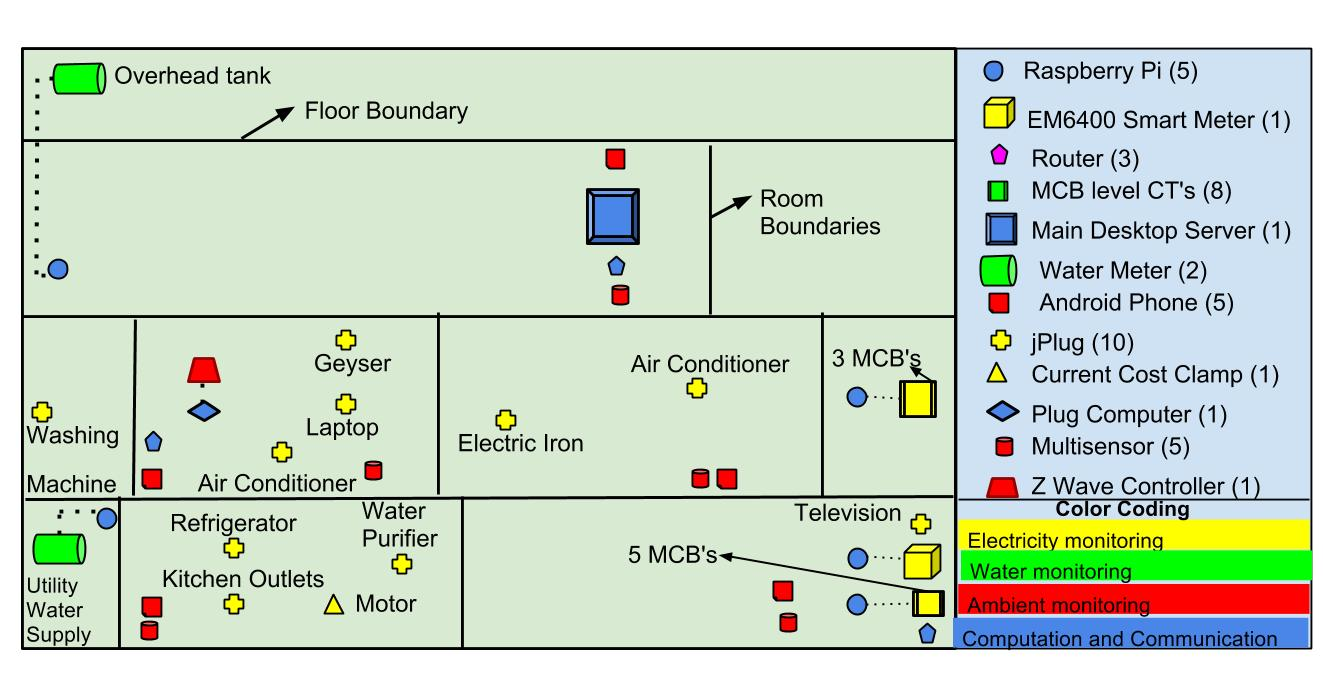
\includegraphics[scale=0.2]{./figures/overall_deployment.jpg}    
    \caption{Schematic showing overall home deployment}   
    \label{fig:overall}
   
\end{figure}
\subsection{Sensing Infrastructure}
\label{sec:sensing}
For our sensing, we took a ``leave no stone unturned'' approach, where  we chose to monitor as many physical parameters (such as ambient conditions, electricity usage, water usage) and non-physical parameters (such as network strength etc.). However, it must be noted, that we chose to deploy sensors in a way that home users can continue their daily routines without getting affected. We describe the various sensors used in our deployments below:

\noindent\textbf{Electricity monitoring:} A typical home electricity setup involves a meter which is installed by utility companies and measures overall electricity usage. Further electric cabling is divided into various Miniature Circuit Breakers (MCB's) which control separate circuits. Typical installations involve putting separate MCB's for heavier loads such as air conditioners and clubbing various lights, fans and other smaller loads into separate MCB. Further each individual appliance is controlled via a switch. There are two types of appliances- i) plug loads like refrigerator and electric iron, which need to be physically ``plugged" into the sockets; ii) loads like lights and fans, which do not need to be ``plugged" in by the user and can directly be switched on or off. We highlight the above described home electricity distribution in \figref{fig:overall}. We have 3 different resolutions at which electricity can be monitored:
\begin{enumerate}
\item \textbf{Meter level:} We use Schneider Electric EM6400\footnote{\url{www.goo.gl/01edPS}} smart meter to instrument the main power supply. While cheaper variants from the same company were available, we chose to use EM6400 as it also provides reactive power. This additional information has been known to be useful for NILM applications\cite{hart}. \figref{fig:em6400} shows EM6400 smart meter deployed in the electricity panel. We had to put 30:5 ratio CT on the power mains coming from the grid to ensure that the load current was transformed to be within EM6400's permissible limits (5 A). EM6400 allows reading various registers to measure more than 40 parameters including: voltage, current, phase, power (apparent, real, reactive) and various other parameters, using Modbus over RS485-serial link.

\item \textbf{Circuit level:} We used our indigenously developed Current transformer (CT) monitor having split core CT's, which can be clamped to indiviual MCB's for monitoring circuit current. This device consists of ADC connected to a low cost microcontroller for sensing max. 8 analog channels simultaneously and pushing computed numerical  values of current from each CT over serial. CT deployment is shown in \figref{fig:ct}.

\item \textbf{Appliance level:} We used jPlug\footnote{A variant of nPlug\cite{nplug}} to measure individual appliance power consumption for 9 plug-load type appliances. We also used Current Cost based CT to measure the power consumption for electric motor (used to pump water), which is not a plug-load, yet has significant power consumption (approx. 700 Watts). jPlug and Current Cost CT deployment are shown in \figref{fig:jplug} and \figref{fig:cc} respectively. jPlug makes a HTTP POST connection to log data. Current Cost exposes apparent power data over the serial port.
\end{enumerate}
More details regarding sensors used for electricity monitoring are provided in \tabref{tab:sensing}.

\noindent \textbf{Water monitoring:} There are few differences in home water distribution in India when compared to developed countries. In India, there are separate water lines for drinkable and non-drinkable water. Also, overhead water tanks (typically 1000 liters capacity) are used to store water. Electric motors are used to push water against gravity to be stored in the tank. Thus, the flow can be summarized as follows: 1) Water from utility comes to the home; 2) Electric motor is used to aid in pumping the water up to the tank; 3) Water flows downward from the tank whenever water is consumed. Thus, we put a water meter at the inlet (coming from the utility) and the outlet from the water tank (flowing downwards) to capture the incoming (from utility) and outgoing (from tank) water consumption. 


Digital water meters are very expensive and are not easily available in India. Thus, we chose to use Zenner Aquamter's multijet\footnote{\url{www.aquametwatermeters.com/multijet.html}}, which are pulse output based water meters, which measure water volume flowing through them. These water meters have a 4 ma current loop \redcolor{Manoj: Add details} and send a pulse every few liters. The precision is based on the quality of the sensor and the diameter of the water pipe. The water meter we used for overhead tank gives a pulse every 10 liters, whereas the one used for inlet supply from utility gives a pulse every 1 liter. These pulses can be measured using the circuit diagram for 4 ma loop shown in ... \figref{fig:water_meter} shows the water meter deployed inline at the overhead tank.

\noindent \textbf{Ambient conditions monitoring:} We used HomeSeer HSM100\footnote{\url{www.homeseer.com/pdfs/guides/HSM100_Release_Notes.pdf}} based multisensors for monitoring motion, light and temperature. While motion is reported in event-driven fashion (i.e. whenever there is change in motion status, reading is reported), temperature and light are polled at 1 Hz. This multisensor uses the well known ZWave\footnote{\url{http://en.wikipedia.org/wiki/Z-Wave}} protocol for communication. We also place Android phones at fixed locations and ran FunF journal\footnote{\url{http://www.funf.org/journal.html}} to log ambient parameters such as light and  sound level.

\noindent \textbf{Miscellaneous:} Android phones, in addition to measuring ambient conditions, were also logging nearby bluetooth and wireless devices and strength of cell-tower signal. All home occupants were requested to keep their phone's bluetooth on during the duration of the experiment. We also logged outside weather conditions such as temperature, humidity and wind speed using publicly available API's from weather monitoring stations. We believe that this data can be used for many applications including: energy-apportionment (i.e. assigning energy usage to different occupants within the home) and localization.

\noindent Sensing infrastructure is summarized in \tabref{tab:sensing}.


\begin{table*}
\caption{Sensing Infrastructure}

\label{tab:sensing}
\tabcolsep=0.015cm
\begin{tabular}{|l|l|l|l|l|l|l|}
\hline
Sensor&Sensor&Sampling&Resolution&Qua-&Commu-&Observed\\
name&type&frequency&&ntity&nication&parameters\\
&&(Hz)&&&&\\
\hline

EM6400&Electric Meter&1&Home&1&RS 485 Serial&Voltage, Current, Frequency,\\ 
&&&&&&Phase, Power(Active, Reactive \\ 
&&&&&&and Apparent), Energy\\ \hline
Aquamet &Water Meter&5&Main supply&2&Direct wire con-&10 liter events for tank and \\ 
multijet&&& and tank&&nection to GPIO&1 liter events for main supply\\ \hline
Homeseer &Ambient multisensors&Light, temperature: 1&Room &6&ZWave&Light, temperature\\ 
     HSM-100           &&PIR: event based&&&& and motion\\ \hline
Android&Ambient multisensors&Audio, light: 0.05&Room&5&Manually&Audio features, light, nearby \\ 
phones&and network&Nearby WiFi, cellular,&&&transfer files&bluetooth, cell-tower, WiFi\\ 
&& bluetooth: 0.001&&&to PC&\\ \hline
Prototype CT&Electricity meter&20&MCB&8&Serial&Current \\\hline
jPlug&Electricity meter & 1 &Appliance&10&WiFi&Voltage, Current, Frequency,\\ 
&&&&&&Power (Active and Apparent),\\
&&&&&& Energy, Phase\\ \hline	
Current Cost&Electricity meter&0.1&Appliance&1&Serial&Apparent power\\ \hline


\end{tabular}


\end{table*}

\subsection{Communication and Computation Infrastructure}
In our experience we found that using a desktop computer for collecting data from sensors would be an overkill in terms of cost, processing power and physical space used. Although microcontrollers are cheap and occupy little space, they do not expose enough abstractions for high level programming and are often difficult to debug and are inherently hard to multi task. We thus decided to use Single Board Computers (SBC's) for sensor data collection. We used Raspberry Pi\footnote{\url{www.raspberrypi.org}} (RPi) and Ionics Stratus\footnote{\url{www.ionics-ems.com/plugtop/stratus.html}} as our SBC's. These SBC's are available for about the same cost (25 \$) as microcontrollers. Moreover, they possess 700 MHz ARM processors and support Linux based distributions. Thus, one can use the full Linux stack and code in higher level languages such as Python. These SBC's run from SD cards whose size can be chosen as per requirement. 

We used a total of 6 SBC's of which 5 were RPi and 1 was Ionics Stratus plug computer. We used a 2 GHz Desktop PC running Linux as the main server where all the data was stored. The software stack running on the SBC's and how they interacted with the main server and collected data from different sensors is described below:

\noindent \textbf{EM6400 smart meter data collection:} EM6400 allows data to be read from its registers over RS485 using Modbus protocol. We connected a RPi to EM6400 using RS485-USB converter which exposes serial interface over USB on RPi. We developed a custom Python program based on pyModbus\footnote{\url{www.github.com/bashwork/pymodbus}} library which would serially read 80 registers, using Modbus protocol, to compute 40 electrical parameters as described in \tabref{tab:sensing}. It would store these 40 parameters along with UTC timestamp in a CSV file. A new CSV would be created every 15 minutes. A background program would periodically try to upload CSV files older than 15 minutes, to the main server, where the data would be dumped in MySQL database.

\noindent \textbf{Current Cost data collection:} Although Current Cost has its own cloud based API platforms, we chose to collect data from it locally, in order to avoid data losses occurring due to network failures. Current Cost provides power data in xml format over the serial interface. We thus connected the USB cable-out from the Current Cost receiver to RPi and wrote a simple Python script to read data serially using pySerial\footnote{\url{www.pyserial.sourceforge.net}} and store it in a CSV file alongwith UTC timestamp. CSV creation and uploading to central server was done in a similar fashion as was done for EM6400.

It must be noted that we used the same model- create new CSV periodically, upload older CSV periodically to main server where they are dumped into MySQL for all sensors. We call this model \paradigms and describe it in more details in section \secref{sec:architecture}

\noindent \textbf{MCB data collection:} Our custom built CT based sensor solution for collecting current data from different MCB's exposes data serially which is read using pySerial on a RPi and processed further using \paradigm.

\noindent \textbf{jPlug appliance data collection:} jPlug makes a HTTP post every second with upto 10 electrical parameters. We saved this data directly on the server machine where a web daemon listened to requests from jPlug and dumped them in MySQL.

\noindent \textbf{Water data collection:} Based on circuitry explained in \secref{sec:sensing}, we used GPIO header on RPi and wrote an interrupt driven program in Python to detect 10 liter and 1 liter events for the tank and supply water meters respectively. We found that noise introduced in the circuit due to long cable lengths led to a lot of false events. Thus, we modified our program and polled at a frequency of 5 Hz to obtain GPIO status and further processed this data using \paradigm.	

\noindent \textbf{Homeseer HSM100 data collection:} We wrote custom wrappers around OpenZWave\footnote{\url{www.code.google.com/p/open-zwave}} program to collect temperature and light information on a per second basis, and motion information based on events. ZWave controller which controls all the ZWave based sensors was connected to the plug computer over USB. Data was processed further using \paradigm. \figref{fig:plug} shows plug computer collecting ambient sensor data from ZWave controller.

\noindent \textbf{Android data collection:} We used FunF journal which would store data inside phone's SD card. We would take a dump once every 15 days and empty the SD card for further data collection.

\noindent \textbf{Weather data collection:} Electricity failure  and reliable Internet are well known problems in India and are highlighted in \secref{sec:learning}. Owing to these problems, we chose to collect weather data from 3 different weather stations, in our collaborator's institute in the USA.

In our deployment a lot of issues pertaining to SBC's were found. For instance, the OpenZWave program that we used would create log files for its own diagnostics. This eventually ate up the 512 MB flash drive space on the plug computer. We fixed this by deleting older logs. This encouraged us to develop soft-sensor streams whereby we collected hard disk space, ping success, CPU utilized, RAM left, temperature of processor for all the computing devices including the server at regular intervals. These soft-sensor streams can be used for alerting mechanisms and can also be used for fault diagnosis. Similar soft-sensor streams have also been used in previous work\cite{hitchhiker_residential} where they used them for alerts.

We found that one WiFi router will not suffice for a 3 storey building. This has also been reported in previous work on residential deployments\cite{hitchhiker_residential}. We thus used 3 routers, where the router on the first floor acted as the host and routers on ground and second floor were bridged to it. More details regarding the need of multiple routers and network availability in homes is described in \secref{sec:learning} and \secref{sec:common}.




\subsection{System Architecture}	
\label{sec:architecture}
Various middleware systems such as sMAP\cite{smap}, Building Depot\cite{buildingdepot} and SensorAct\cite{Arjunan12} have been proposed in the past for sensor data collection. However, we found that they are not fine tuned to our needs arising from faulty internet, power failures, etc. Moreover, these systems provide a lot more features than we intend to use. Thus, based on our experience and previous work\cite{hitchhiker_residential}, where importance of simplifying the architecture are proposed, we propose \paradigm. \paradigms involves local storage and periodic data upload. As explained above, we used SBC's to collect data from sensors. This data was \textbf{locally stored} in form of comma separated value files (CSV) and was \textbf{periodically uploaded} to the main desktop server. In case the upload failed, it was retried the next time again. Each SBC had sufficient flash based local storage to accommodate sensor data for a few days. 

\begin{figure}     
    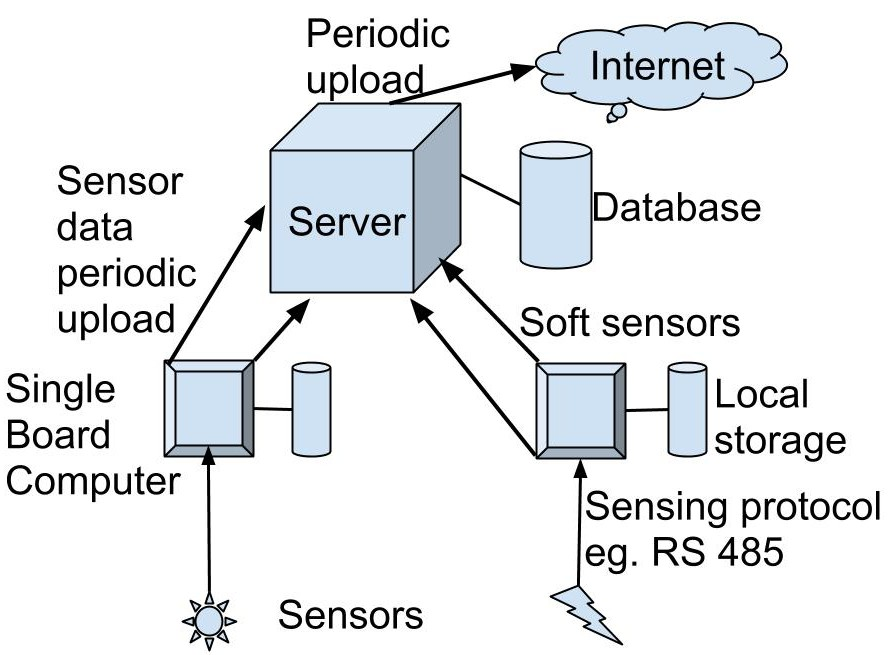
\includegraphics[scale=0.20]{./figures/architecture.jpg}    
    \caption{\paradigm}   
    \label{fig:architecture}   
\end{figure}

\begin{figure}  
\subfloat[\scriptsize Different resolutions of measuring electricity consumption in home]{
	 \label{fig:electricity_distribution}
    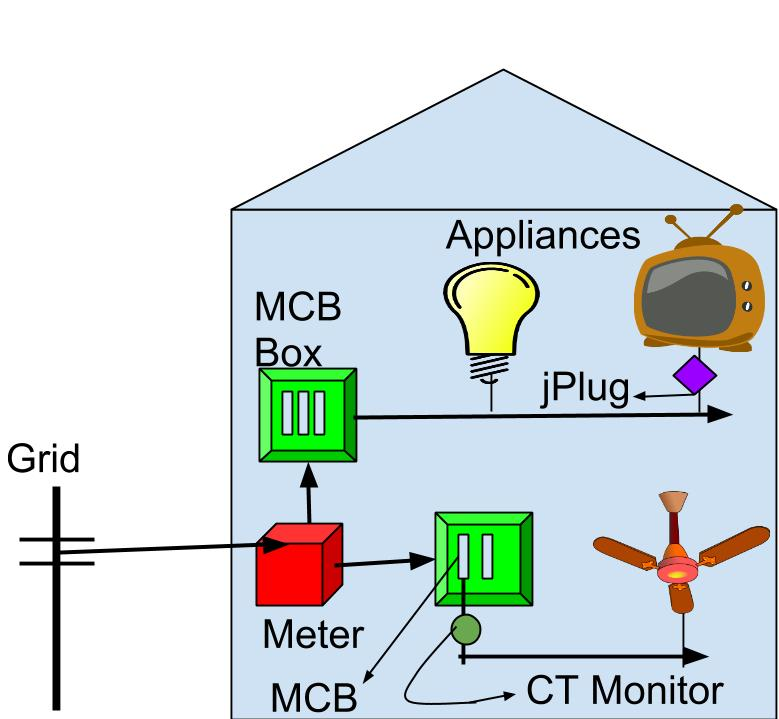
\includegraphics[scale=0.14]{./figures/electricity_distribution.jpg}}
    \hspace{1mm}
    \subfloat[\scriptsize Different resolutions of measuring water consumption in home]{
    	 \label{fig:water_distribution}
        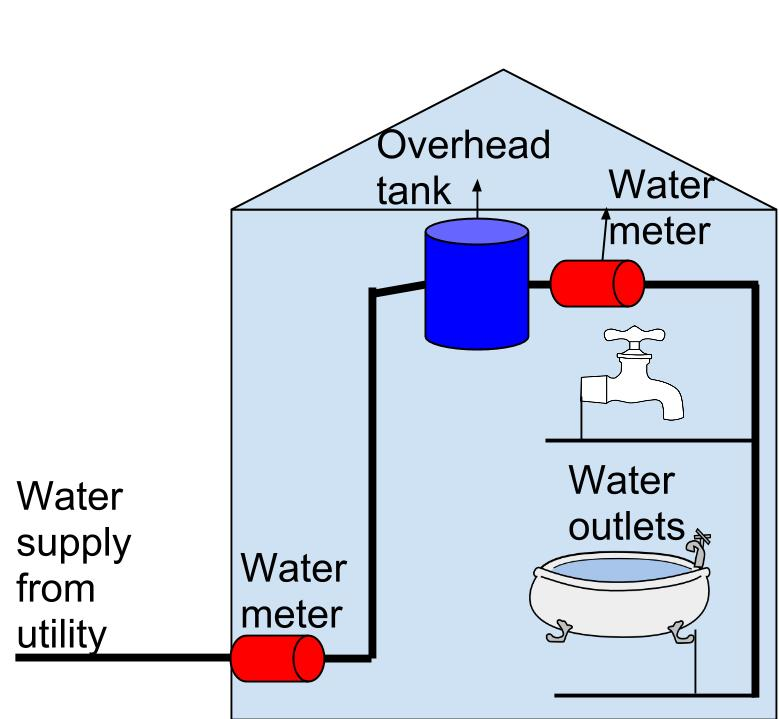
\includegraphics[scale=0.14]{./figures/water_distribution.jpg}}
    \caption{Different resolutions of measuring electricity and water consumption in home}   
      
\end{figure}



Web applications running on the server allowed a home user to locally visualize his data from multiple streams. Further, data from the server can be copied to cloud based servers such as Dropbox where applications such as analytics, alerts can be done, allowing outside users and specifically researchers to keep an eye on the deployment sitting in their labs. \figref{fig:architecture} explains \paradigms architecture. The salient features of our architecture are as follows:
\begin{itemize}
\item \textbf{Decoupled sensing and data uploading:} This ensures that an error in one does not prevent the other action from occurring correctly and thus allows easier debugging. Moreover, this design choice of decoupling comes from the well established principles of software engineering.
\item \textbf{Minimal internet requirement:} Internet is required \textbf{only} when outside researchers wish to view and analyze collected data in realtime. Internet failure does not have any impact on sensor data collection.
\item \textbf{Reduced load on server:} Since data is uploaded periodically in larger chunks rather than sending data for each sensor packet, computation and bandwidth requirements are greatly reduced.
\end{itemize}

\begin{figure*} 
    
    \subfloat[\scriptsize EM6400 Smart Meter]{
    \label{fig:em6400}
    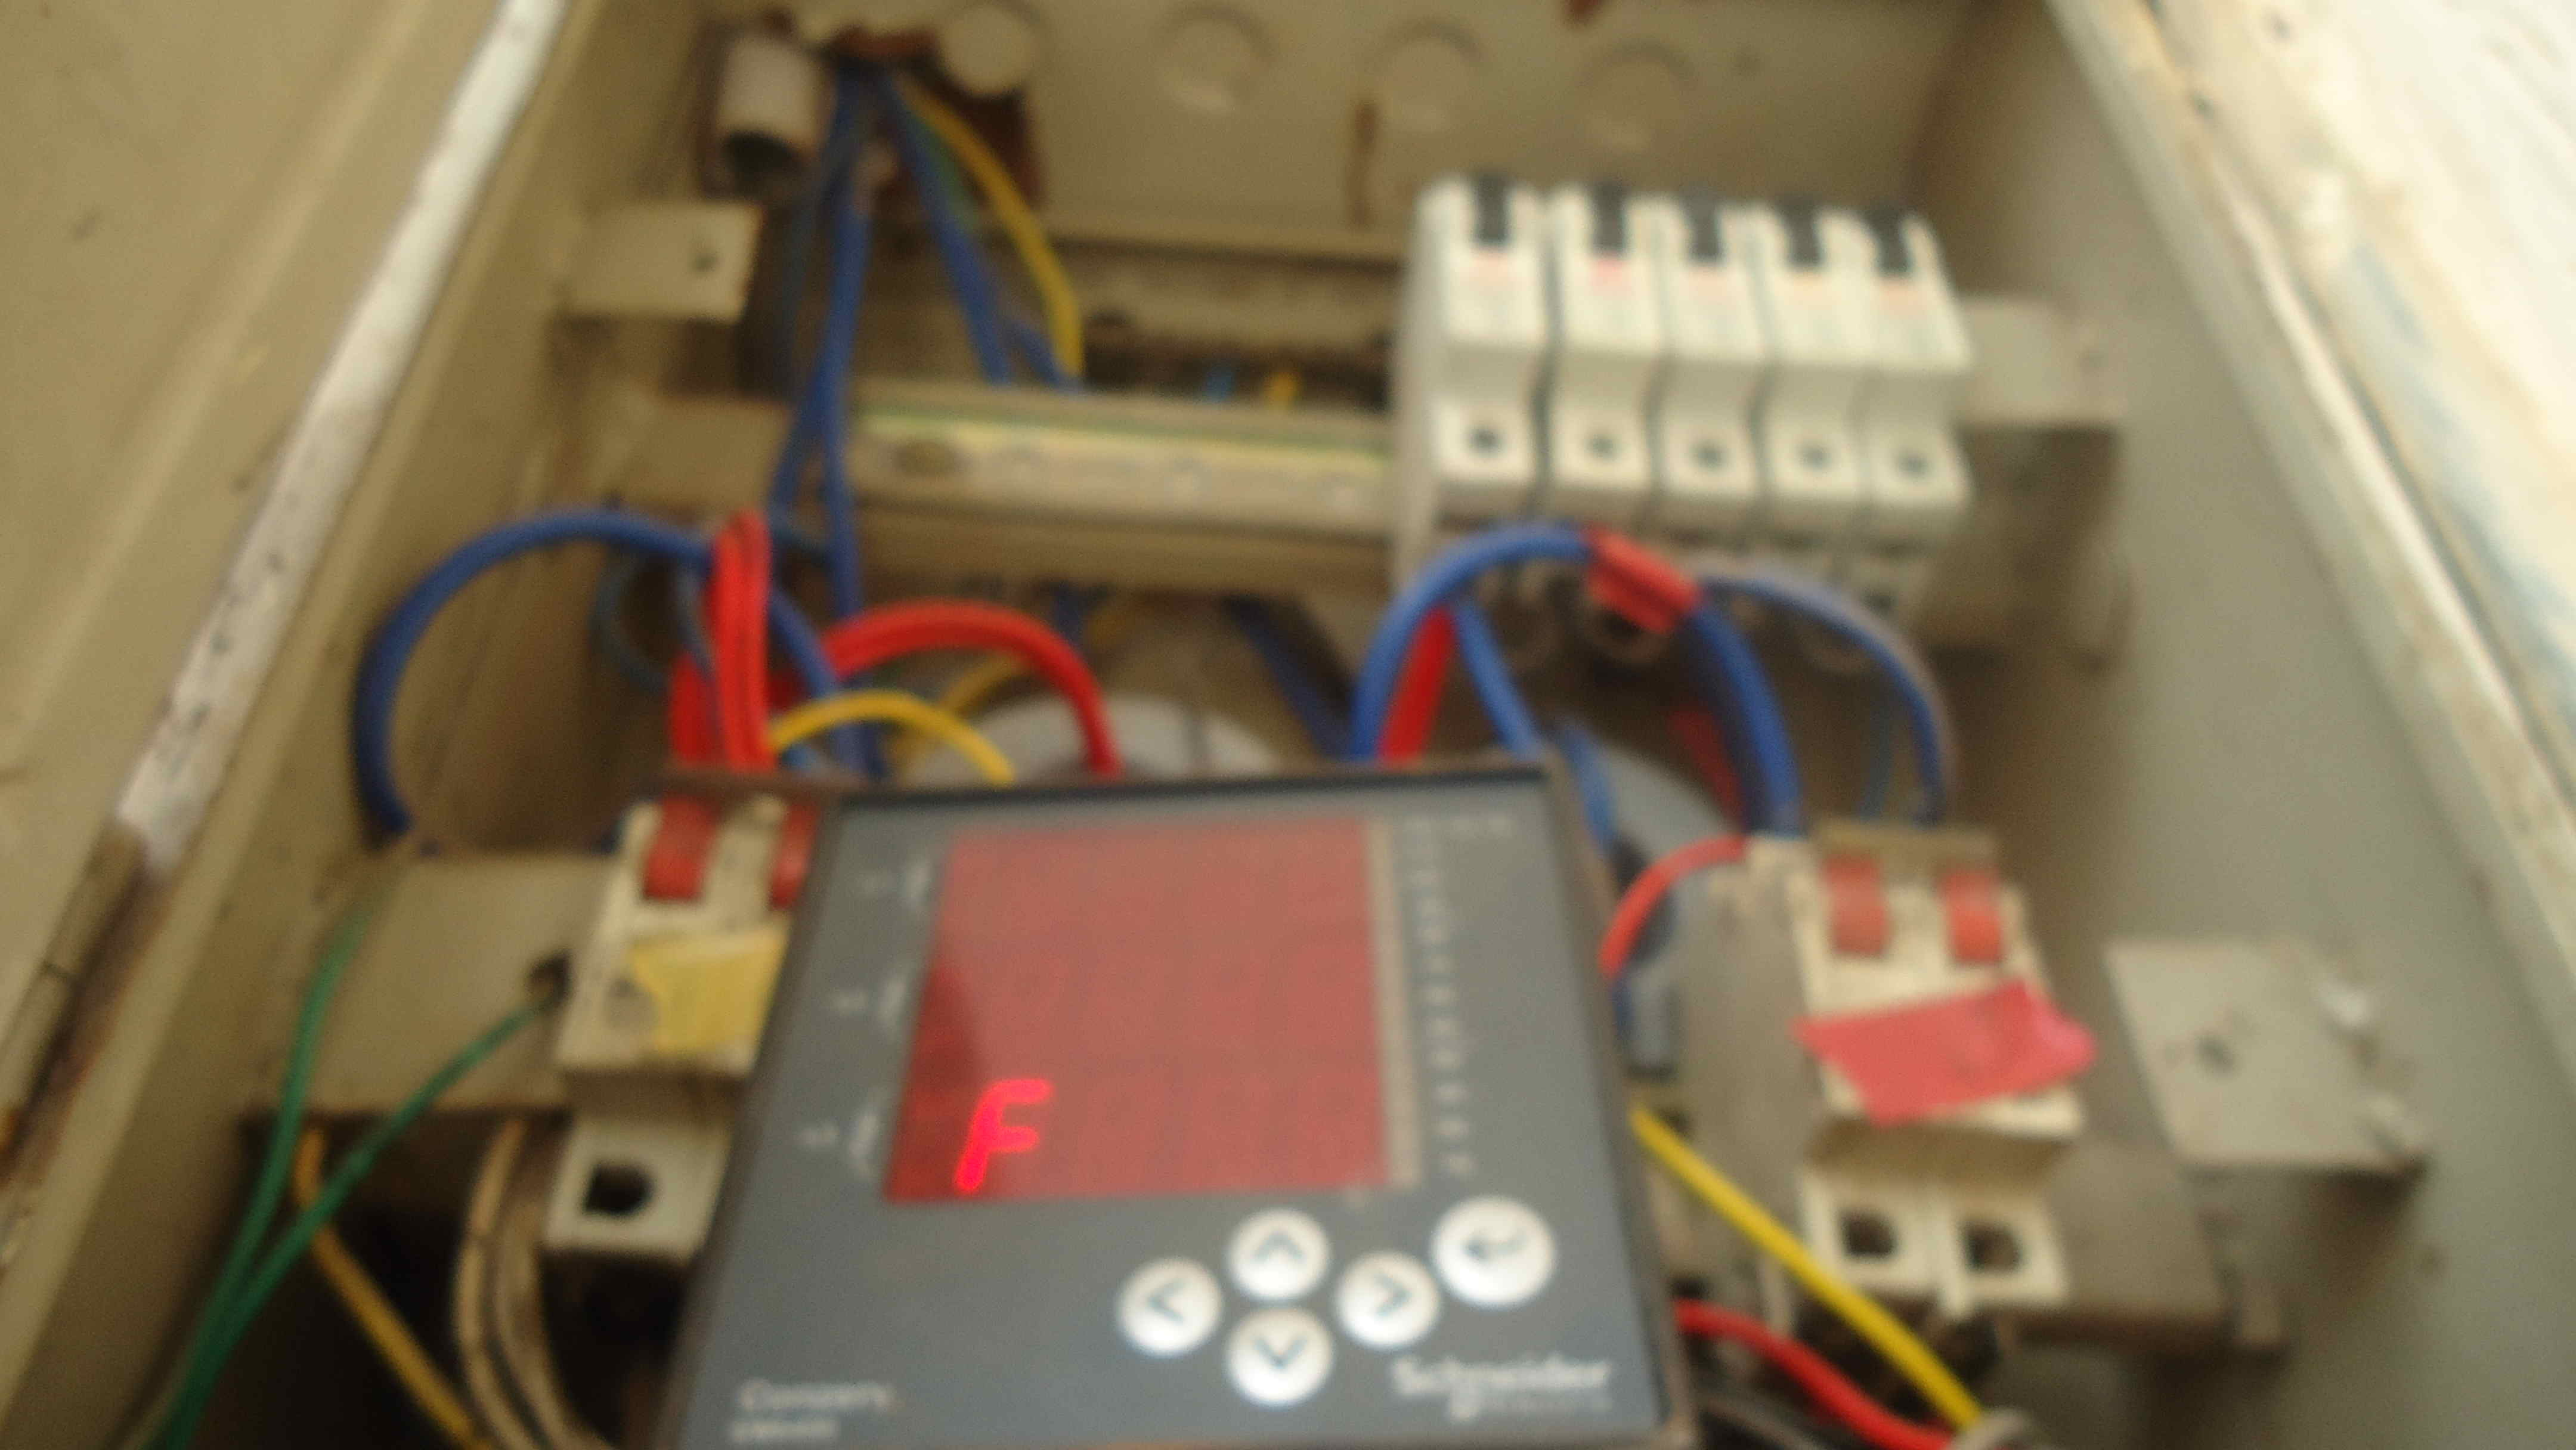
\includegraphics[scale=0.027]{./figures/electric_meter_2.jpg}}
    \hspace{1mm}
     \subfloat[\scriptsize In-house developed CT monitoring system for measuring current data from MCB's]{
        \label{fig:ct}
        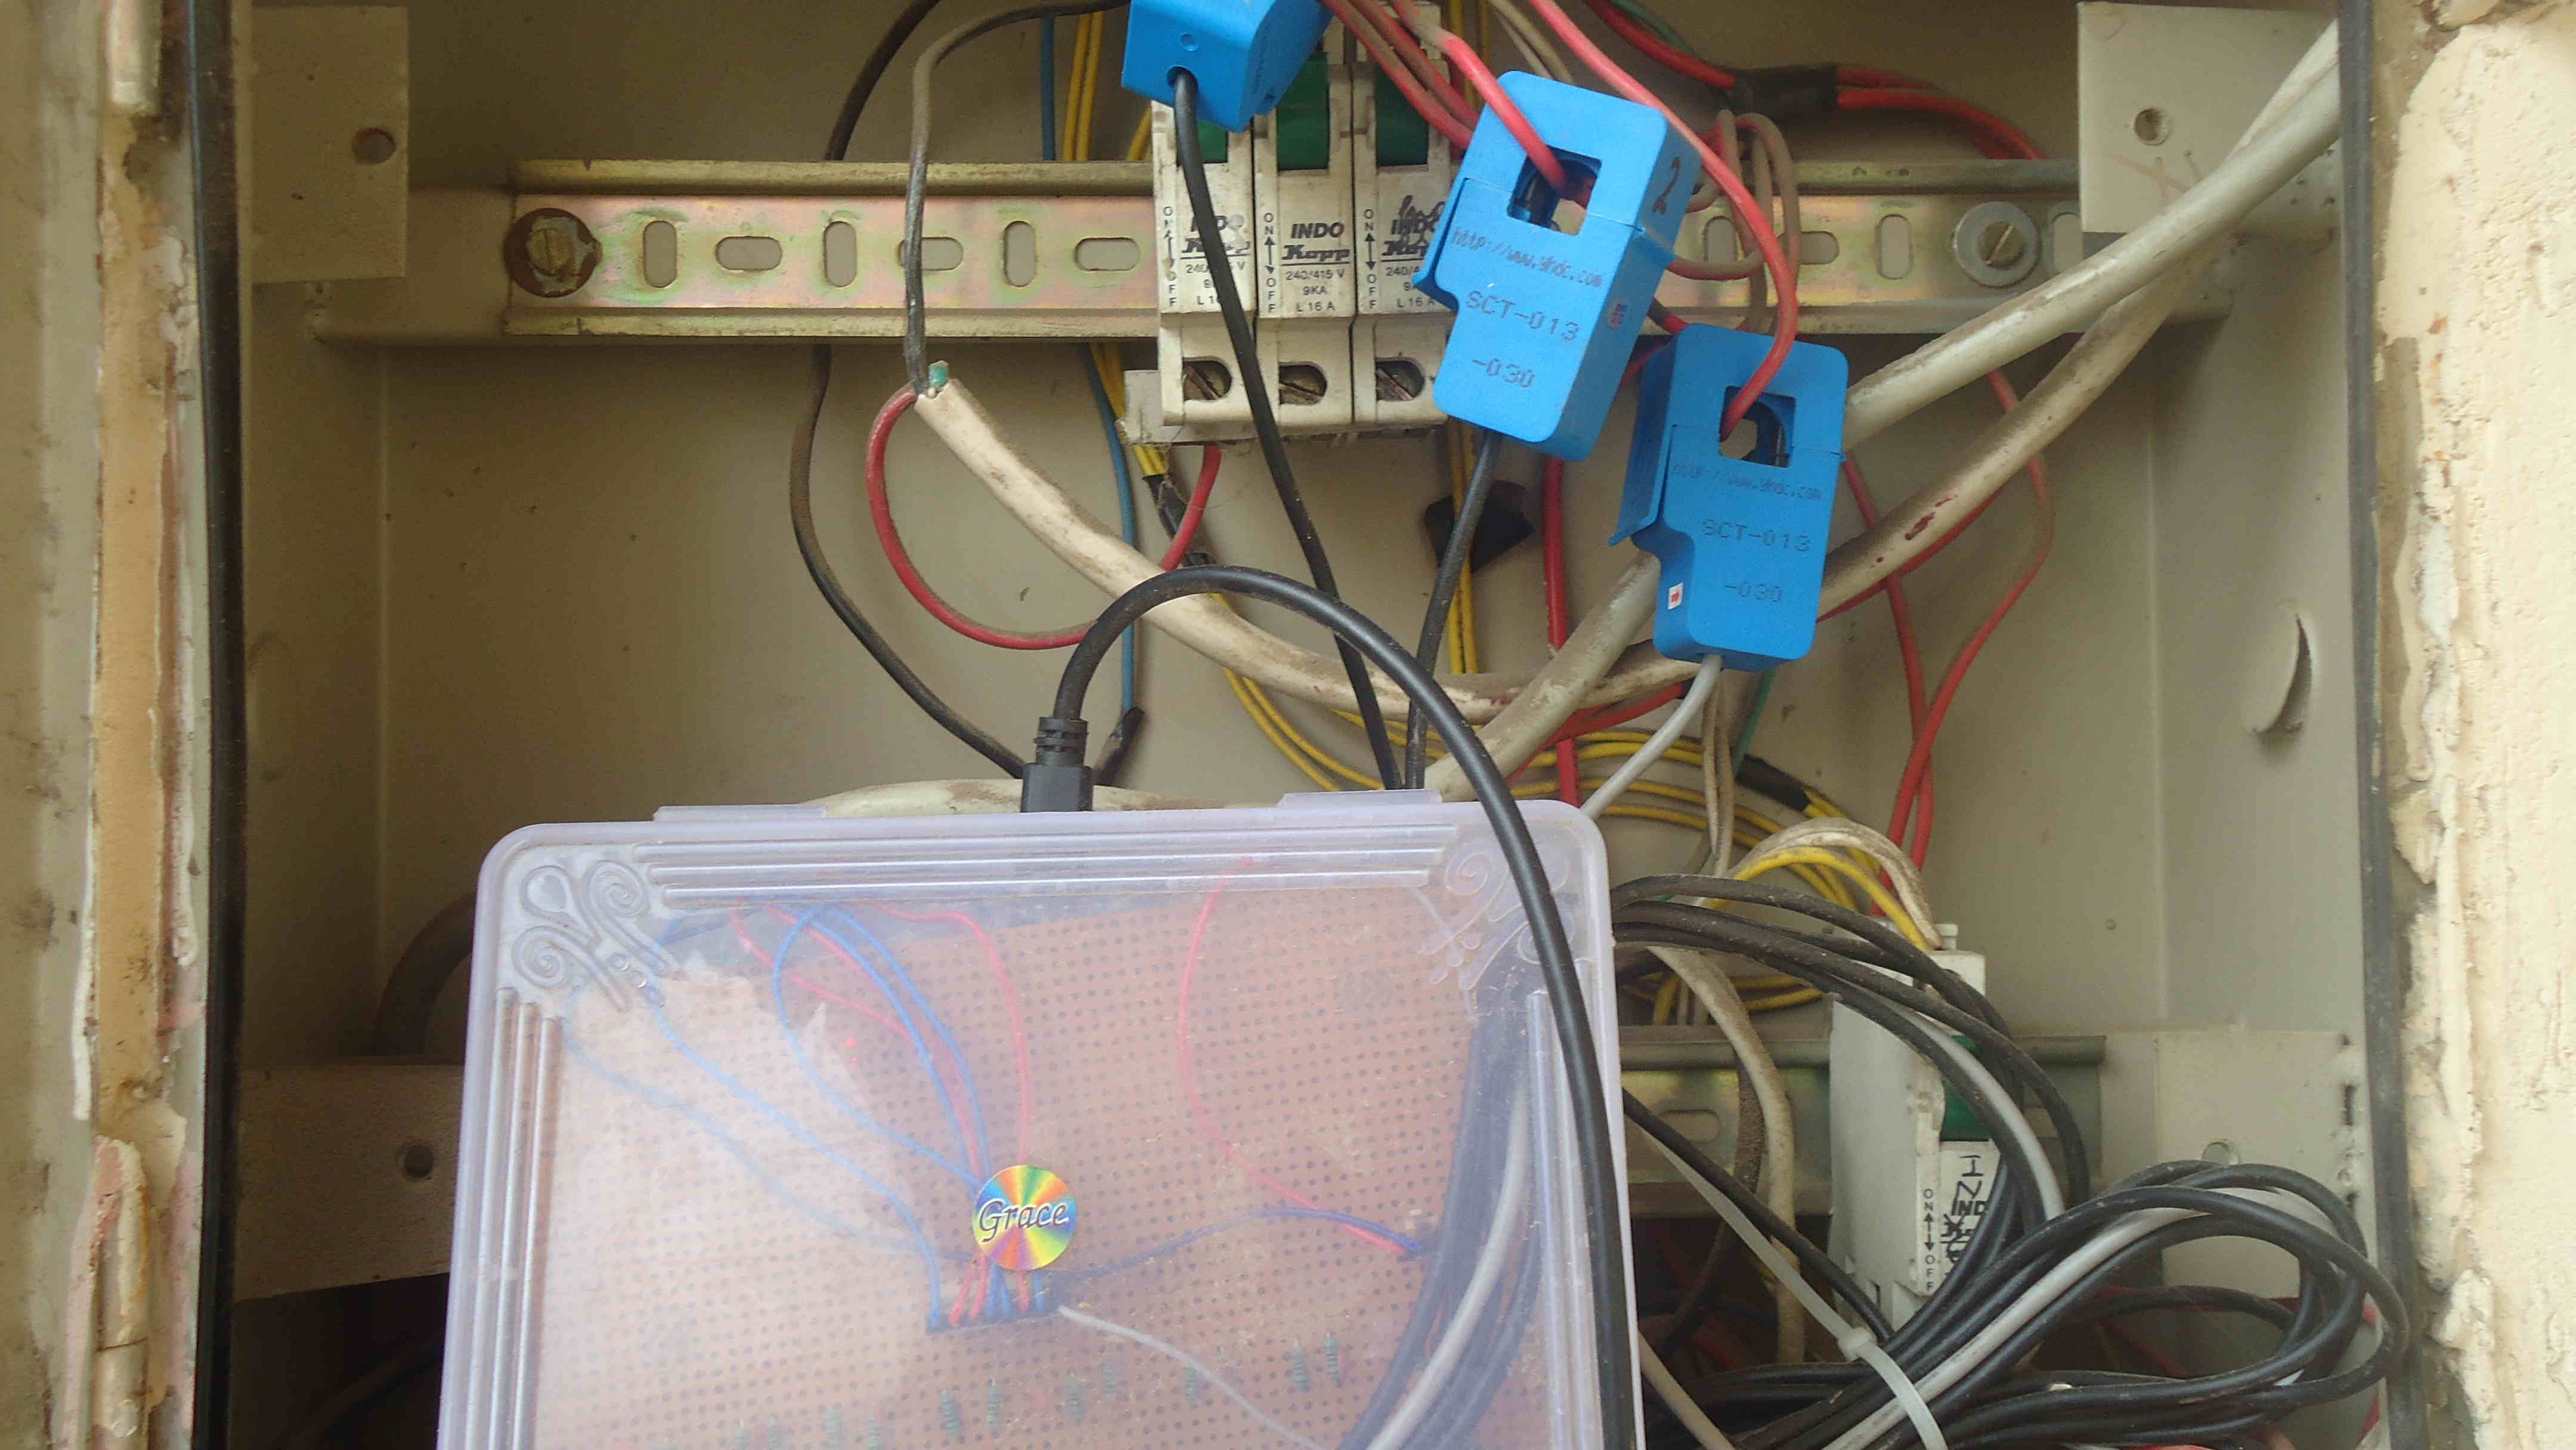
\includegraphics[scale=0.027]{./figures/mcb.jpg}}
       \hspace{1mm}
     \subfloat[\scriptsize Appliance level monitoring using jPlug]{
             \label{fig:jplug}
             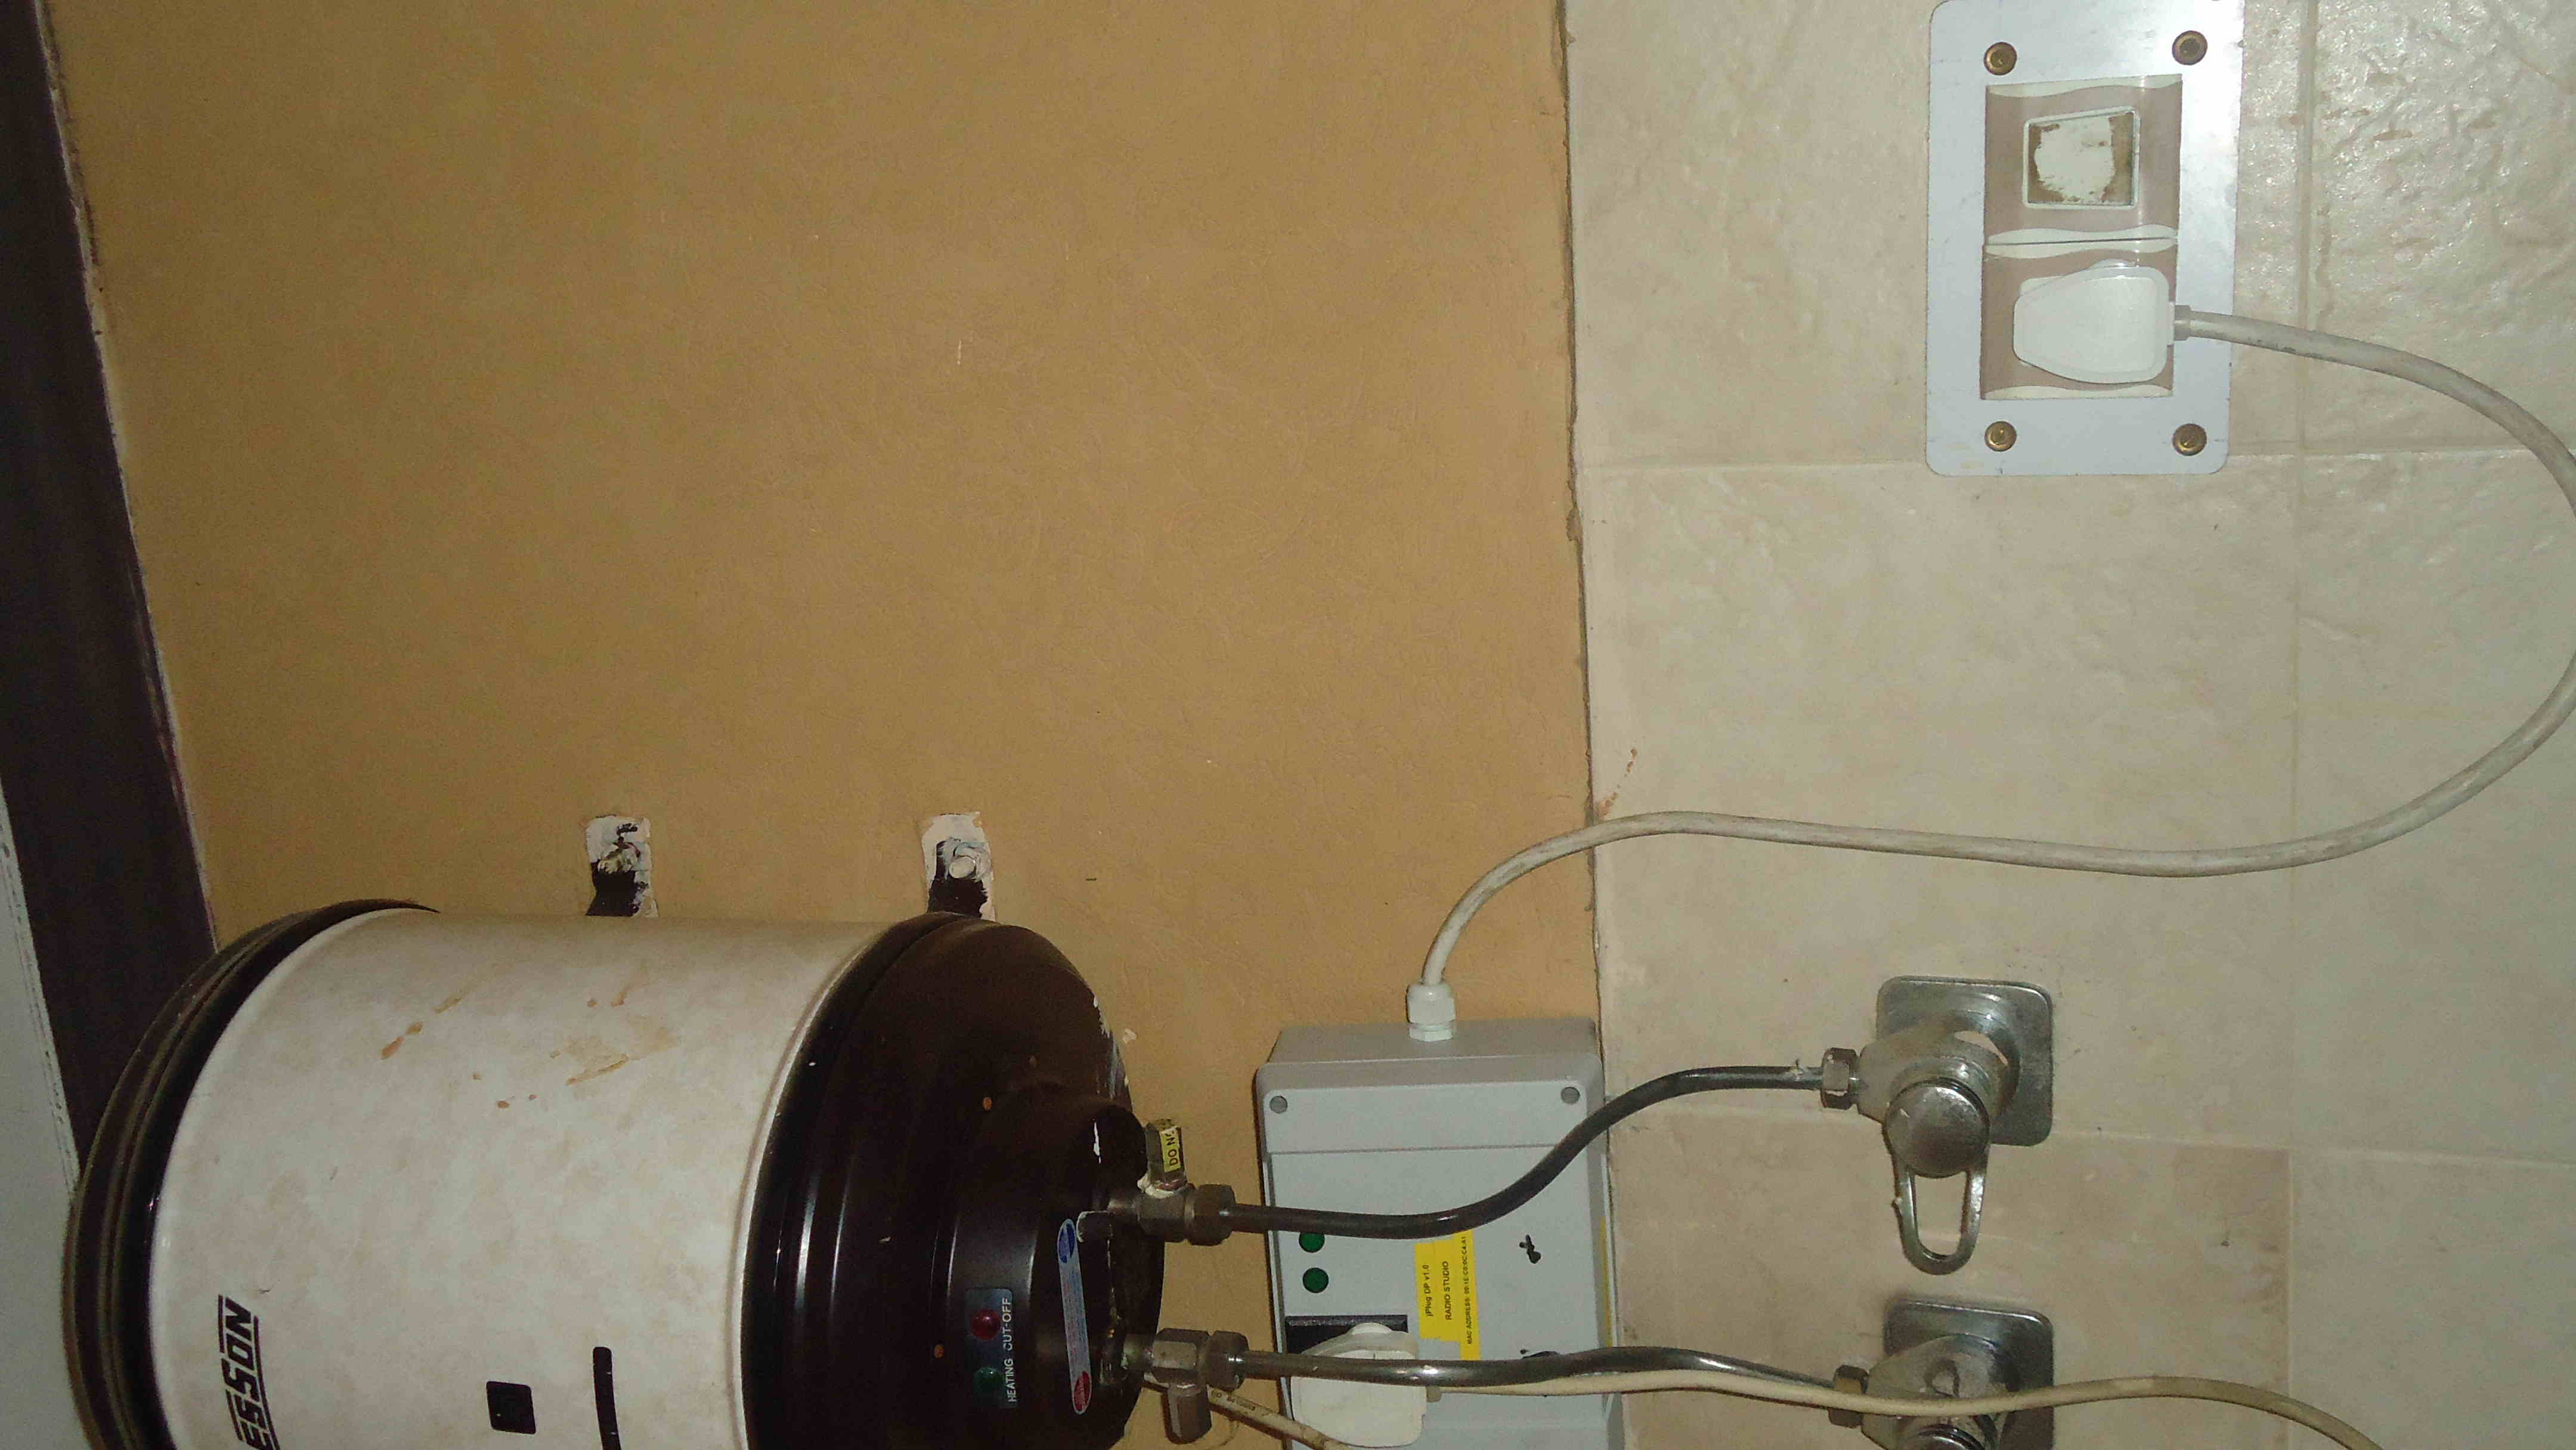
\includegraphics[scale=0.027]{./figures/jplug.jpg}}
             \hspace{1mm}
          \subfloat[\scriptsize Appliance level monitoring using Current Cost CT]{
                  \label{fig:cc}
                  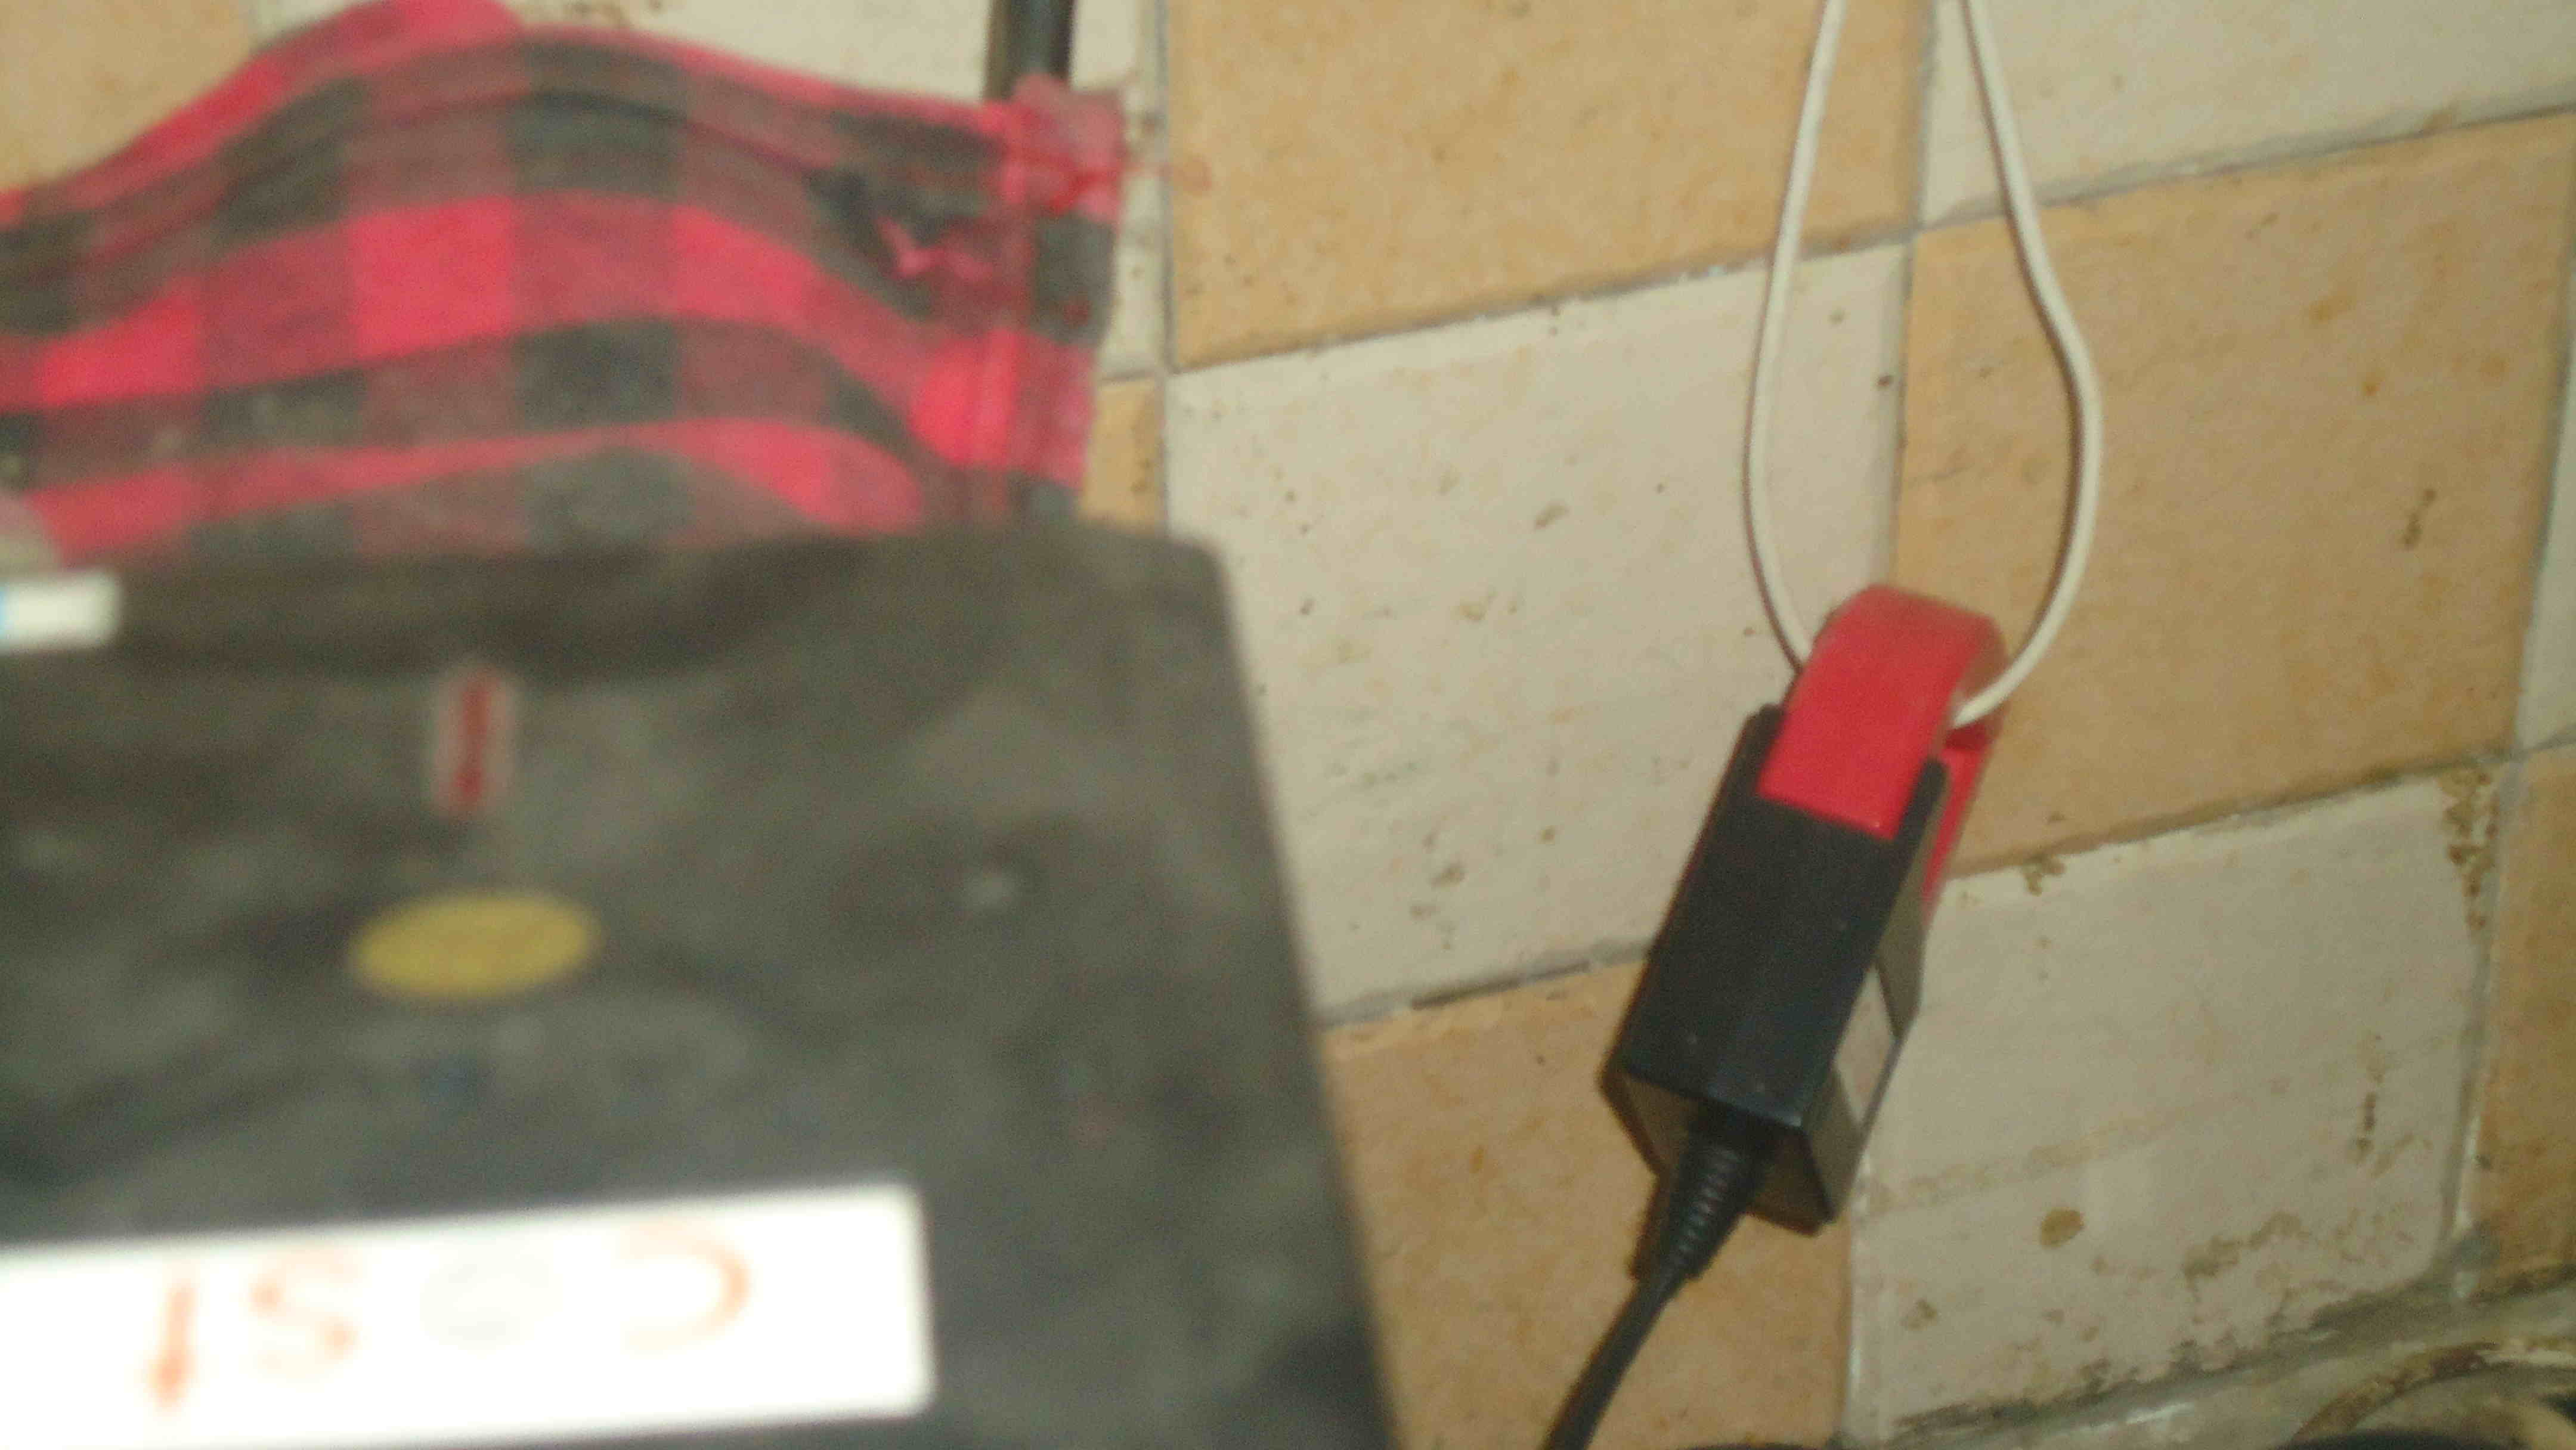
\includegraphics[scale=0.027]{./figures/cc.jpg}}
    %\hspace{0.02\columnwidth}
    \newline
    \vspace{-2mm}
    \subfloat[\scriptsize Water Meter]{
    \label{fig:water_meter}
        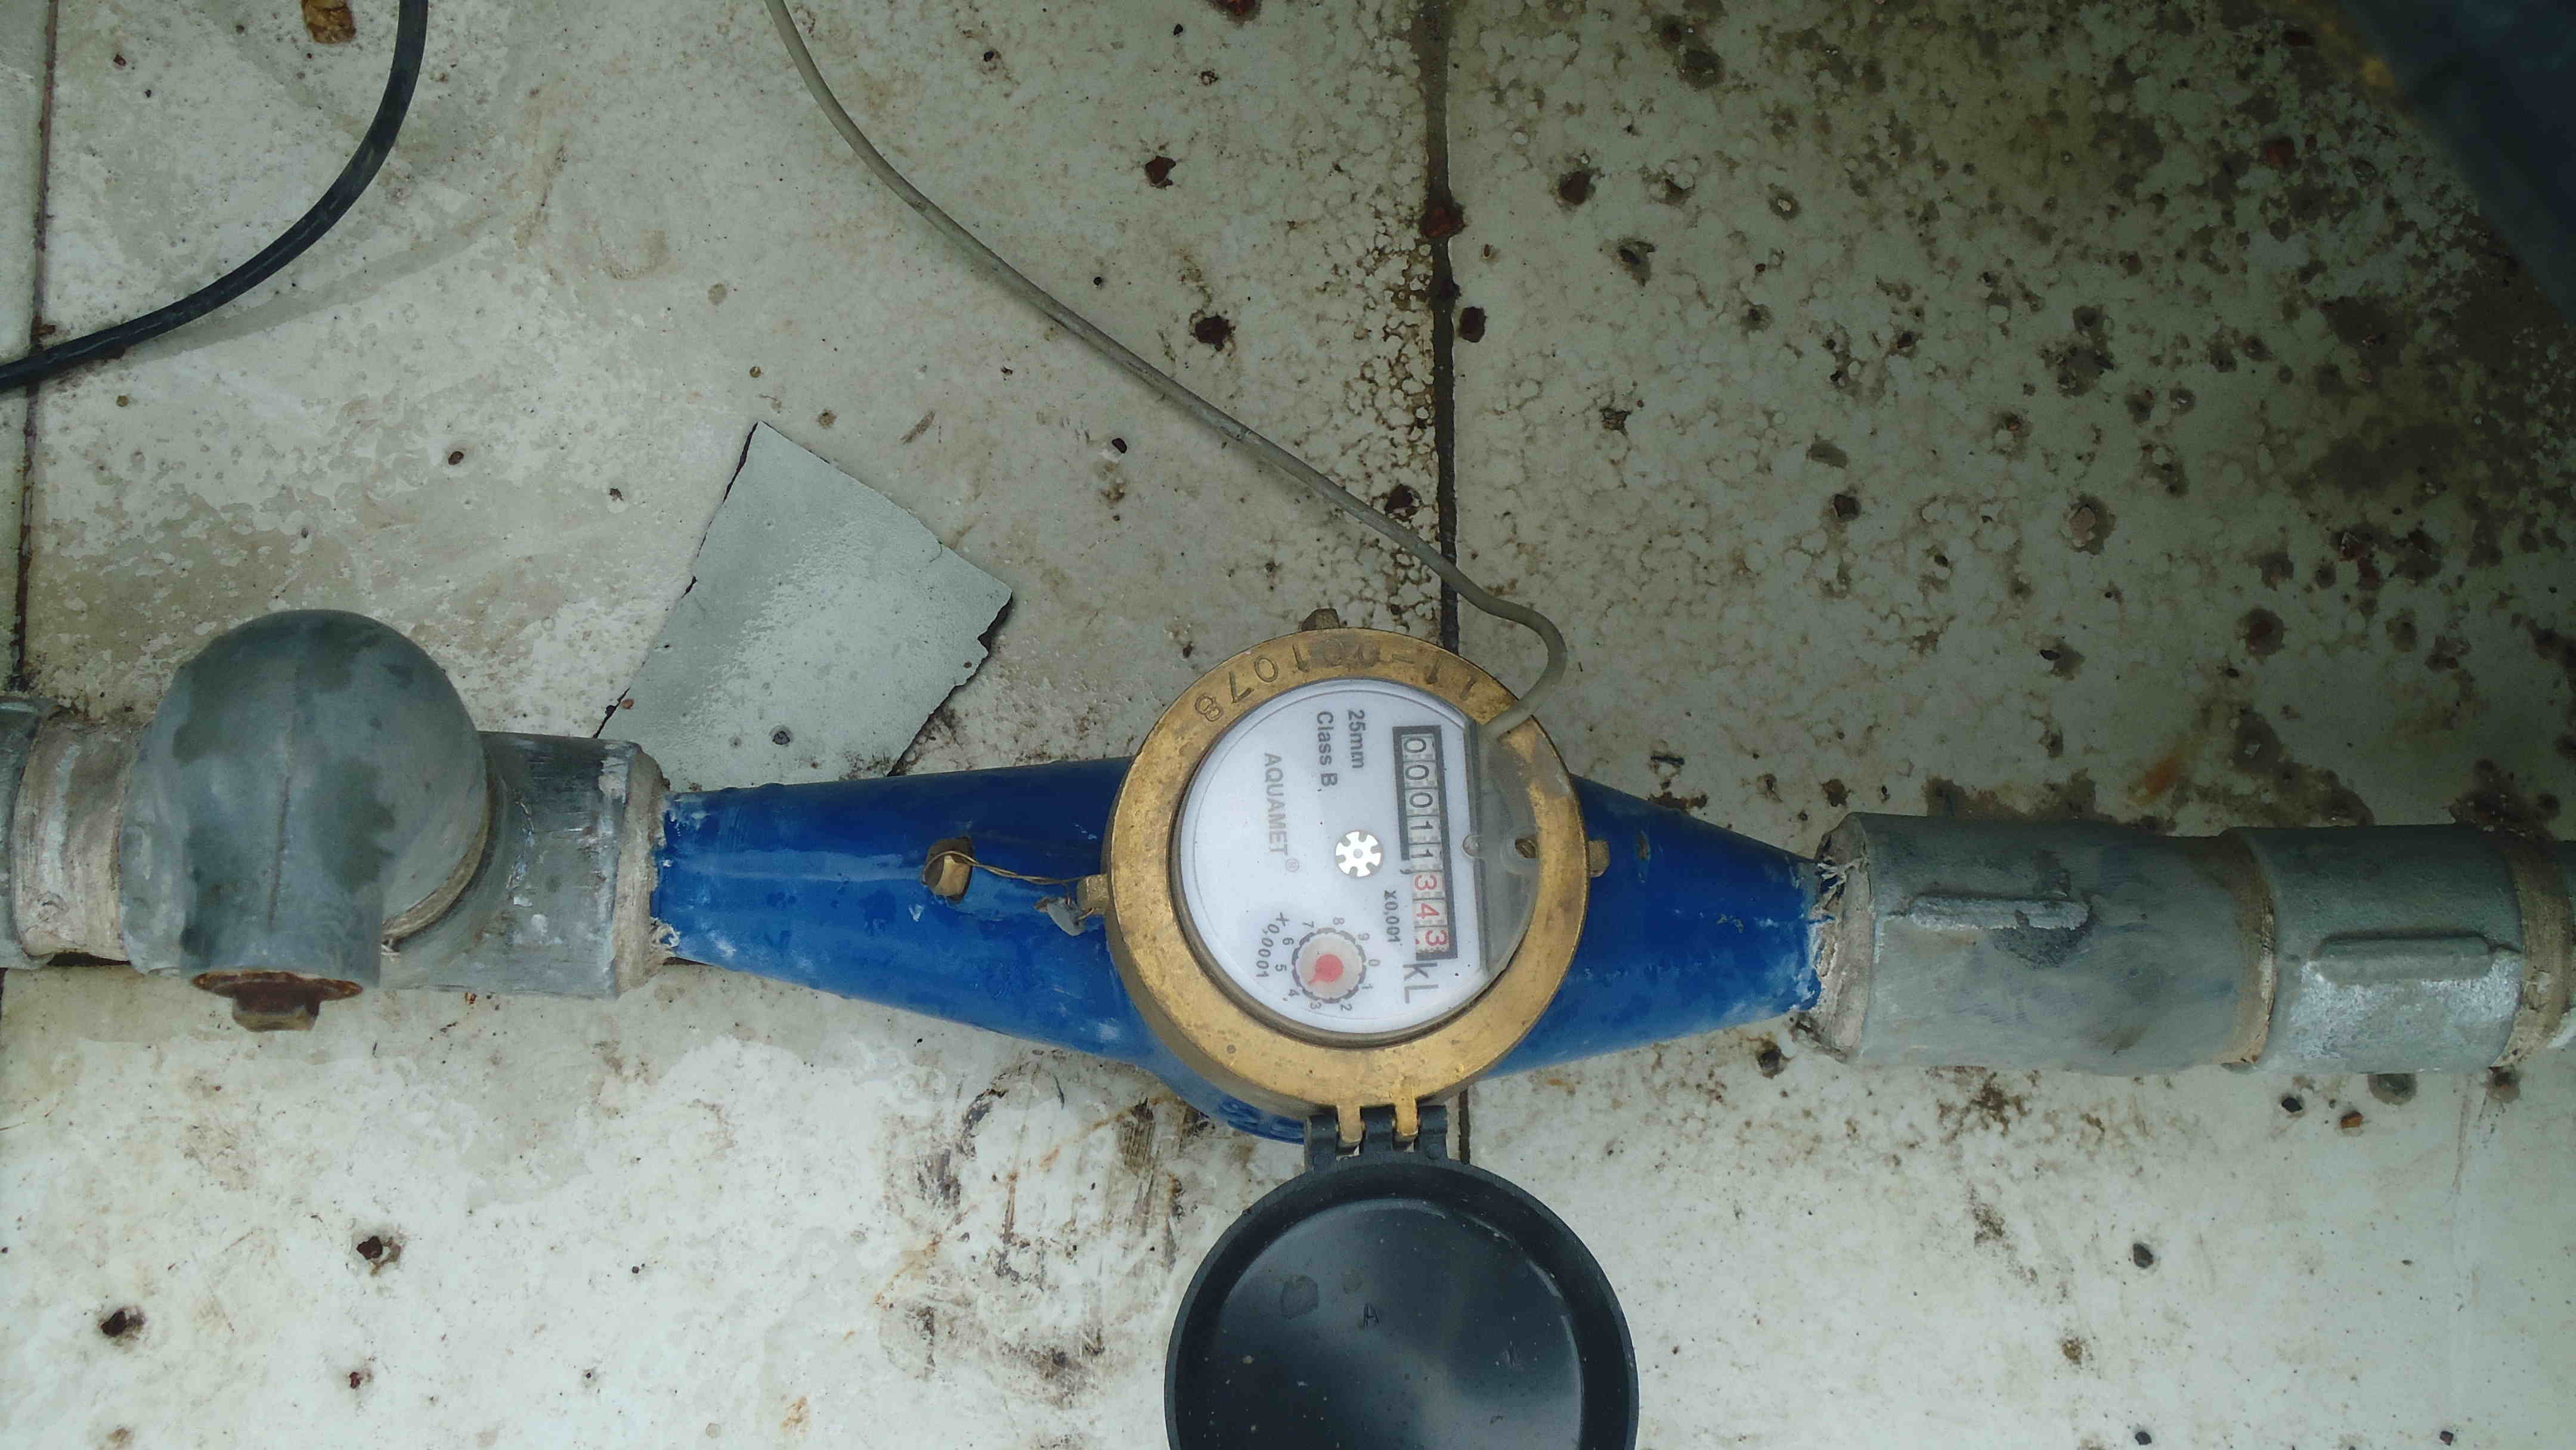
\includegraphics[scale=0.027]{./figures/water_meter.jpg}}
        \hspace{1mm}
     \subfloat[\scriptsize Android phone and Homeseer Zwave multisensor used to measure ambient parameters]{
        \label{fig:ambient}
            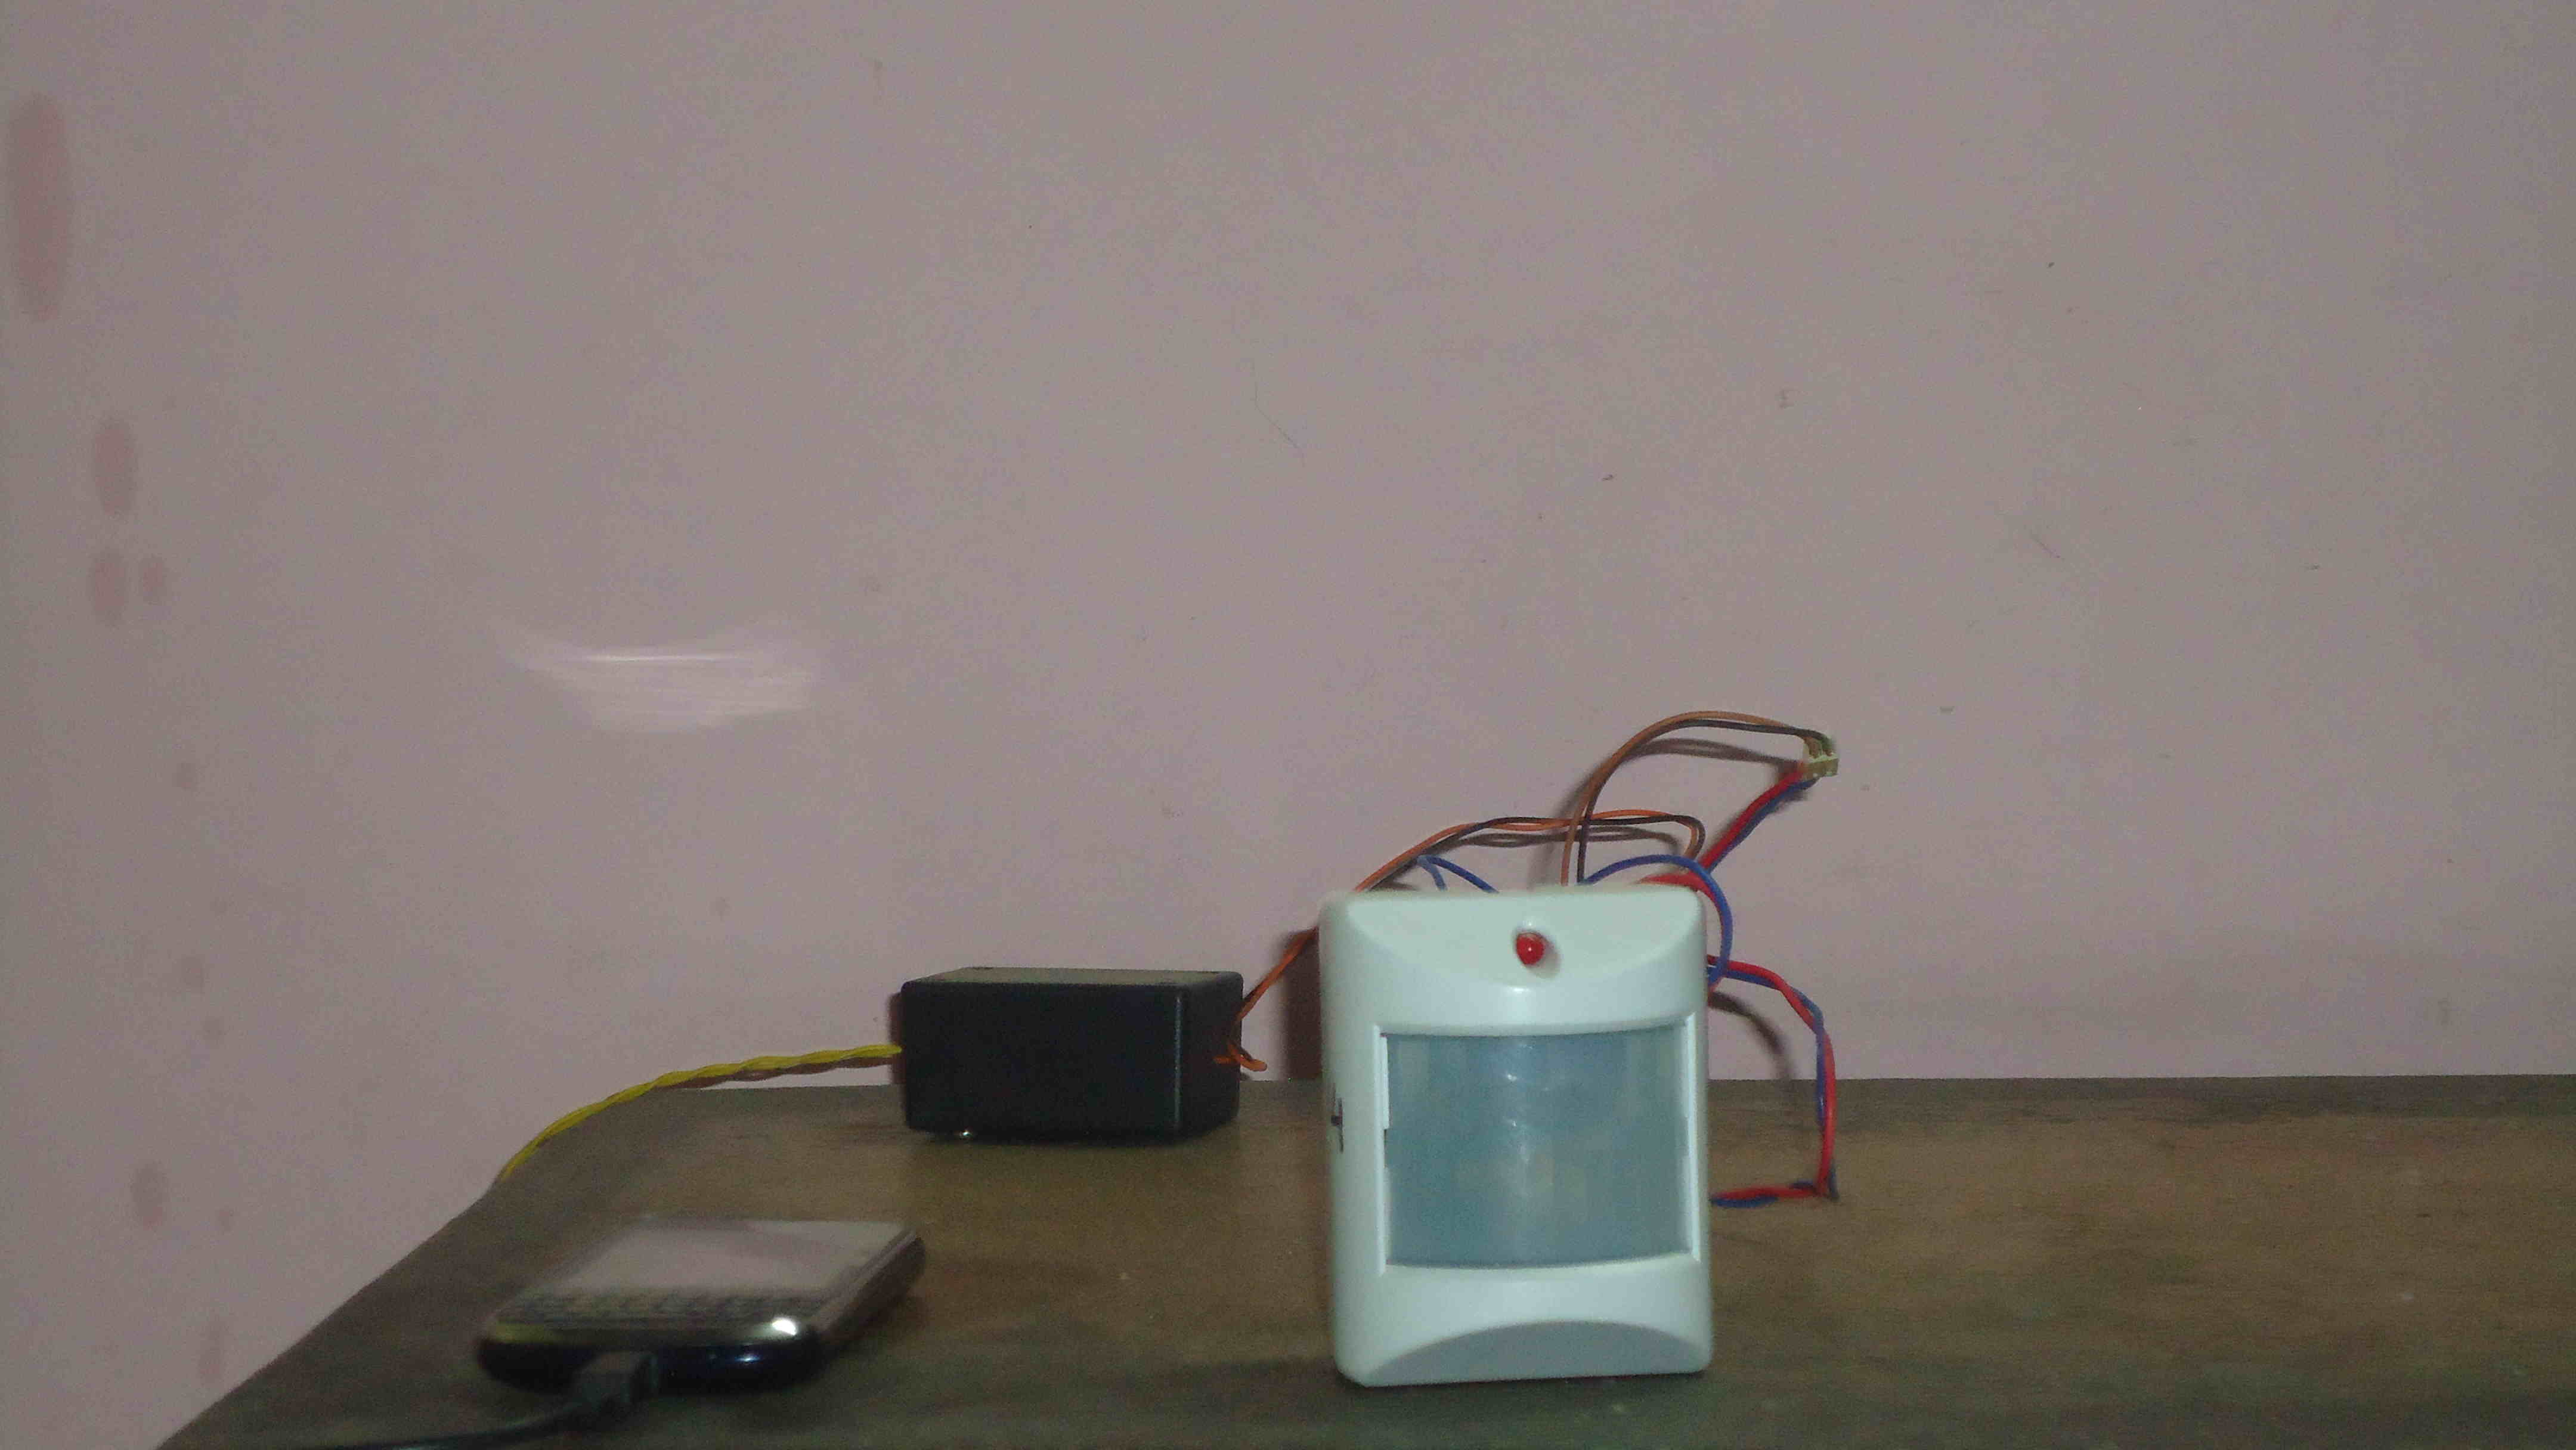
\includegraphics[scale=0.027]{./figures/ambient.jpg}}
            \hspace{1mm}
       \subfloat[\scriptsize Plug computer collecting data from ZWave controller and connected to the router via an ethernet cable]{
              \label{fig:plug}
                  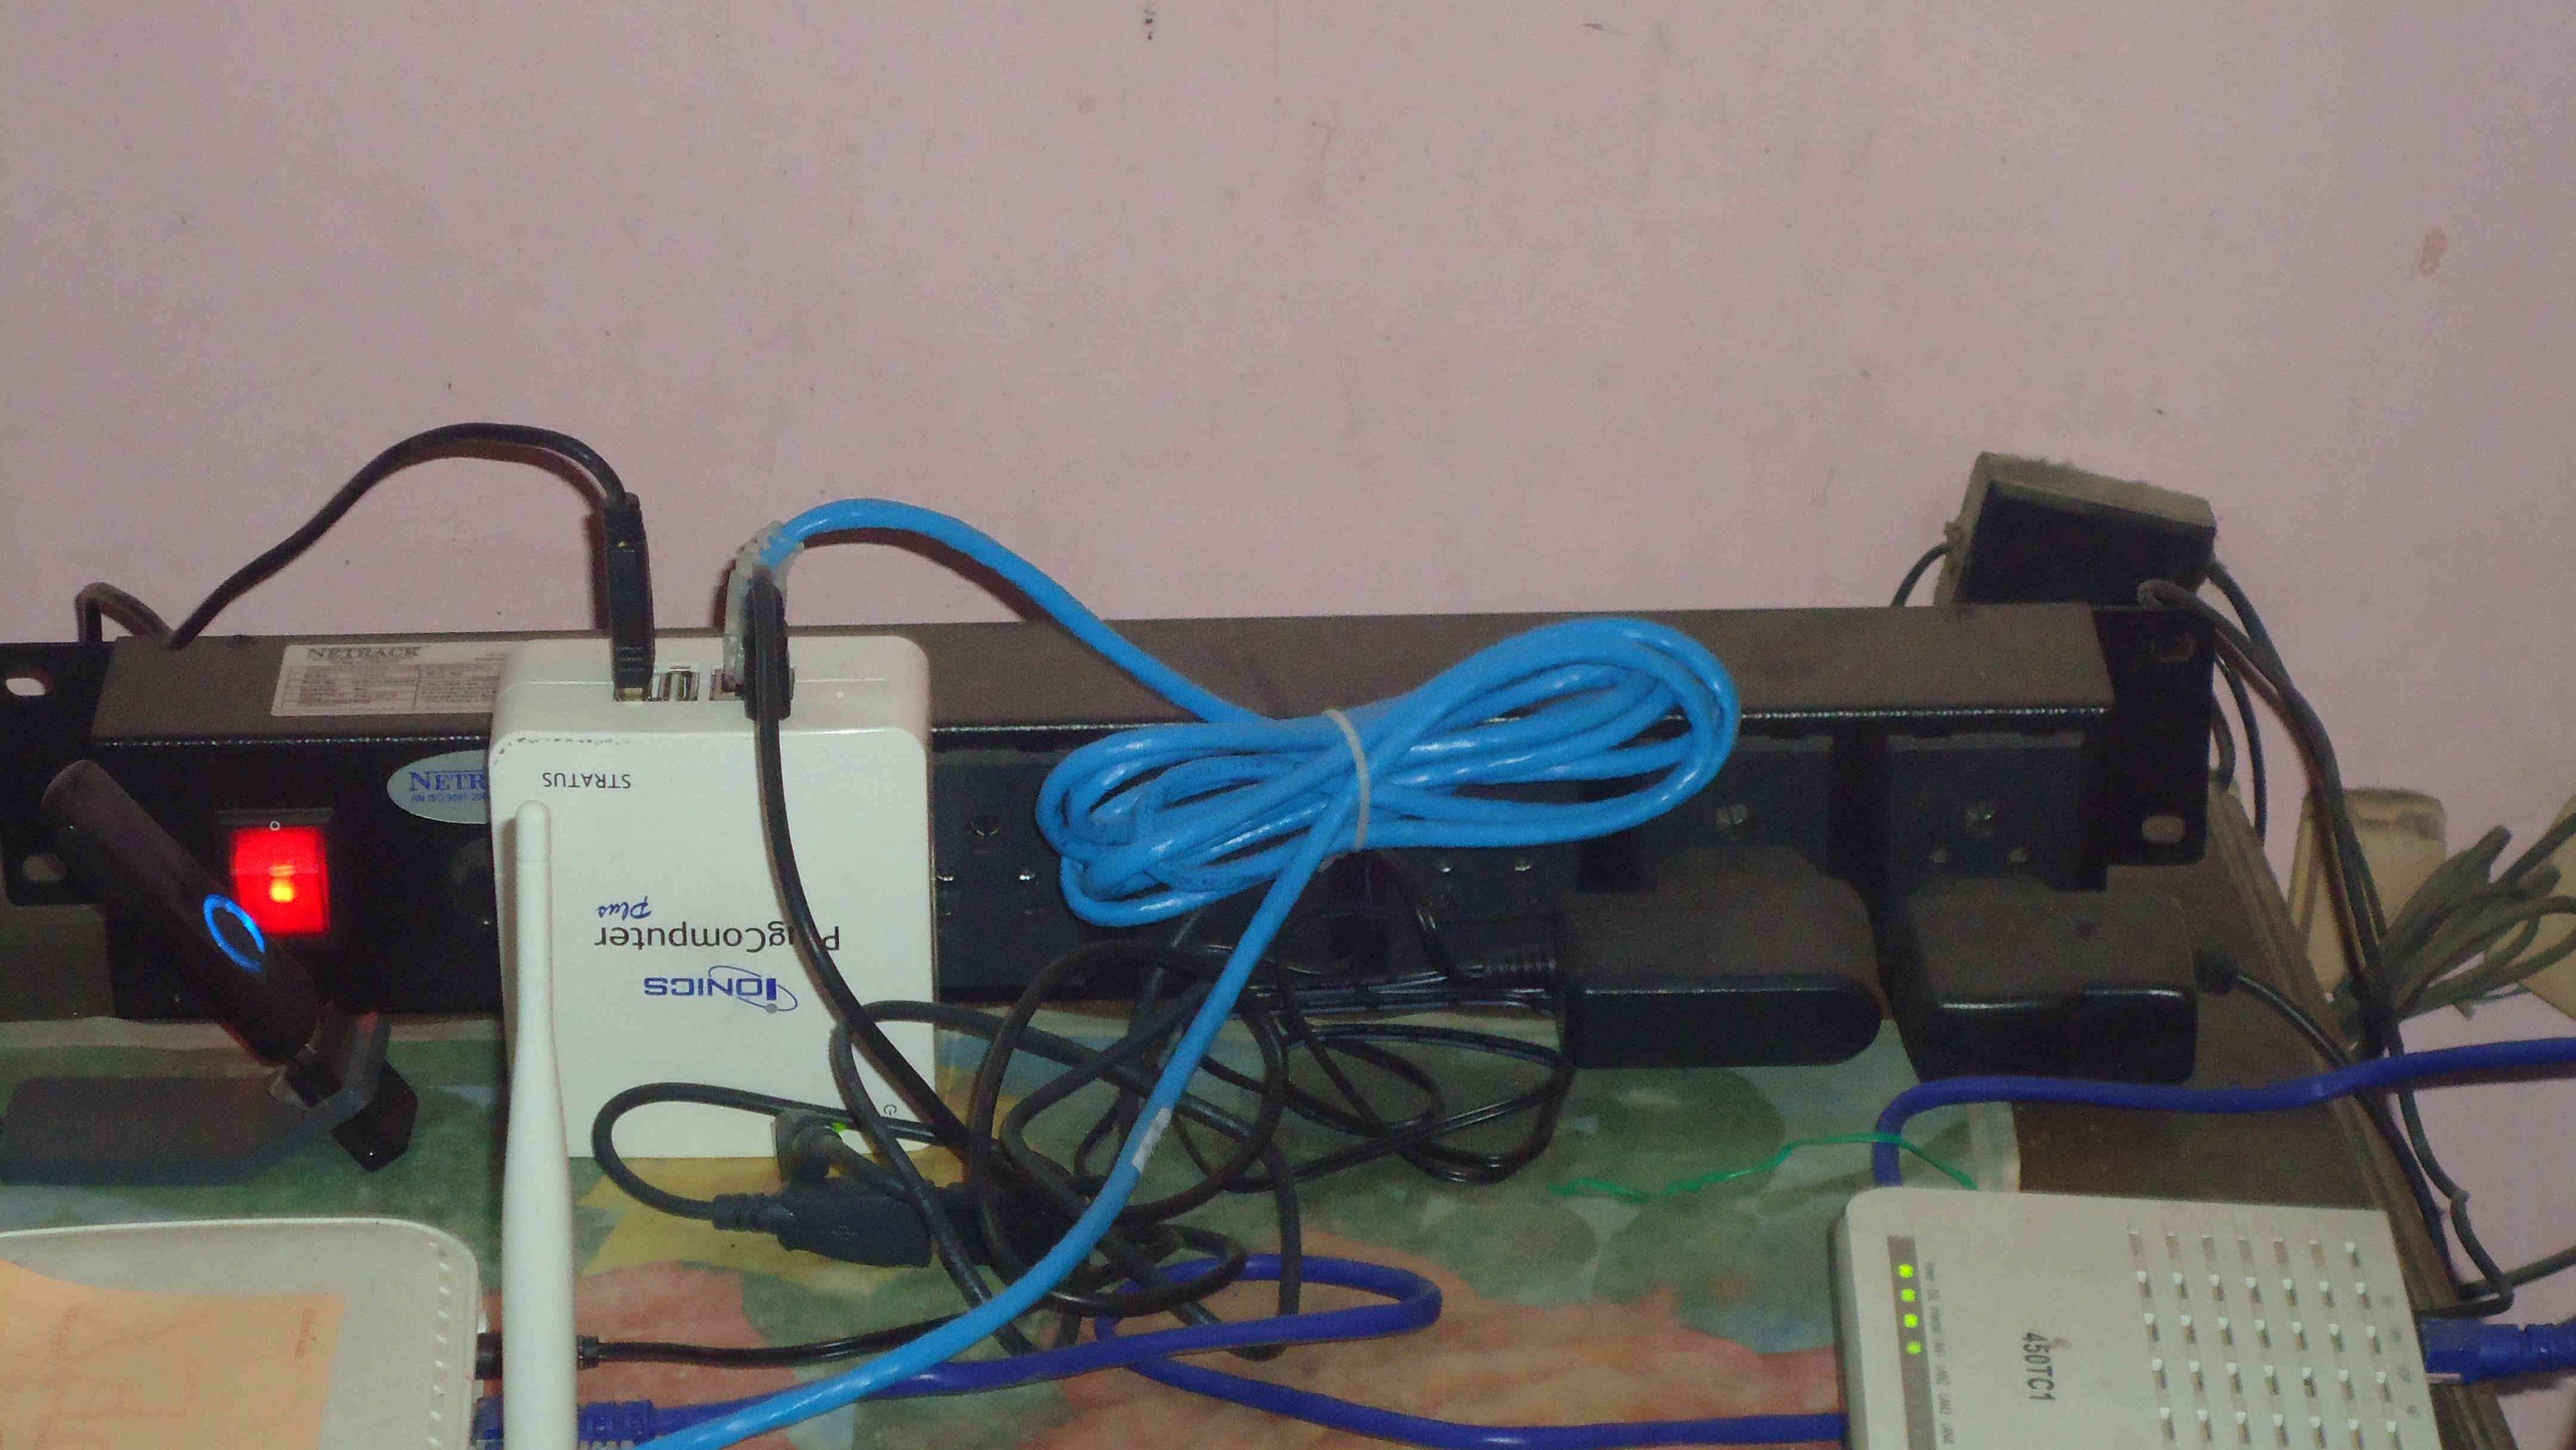
\includegraphics[scale=0.027]{./figures/plug.jpg}}
                  \hspace{1mm}
         \subfloat[\scriptsize RPi collecting water meter data using GPIO pins]{
                     \label{fig:rpi}
                         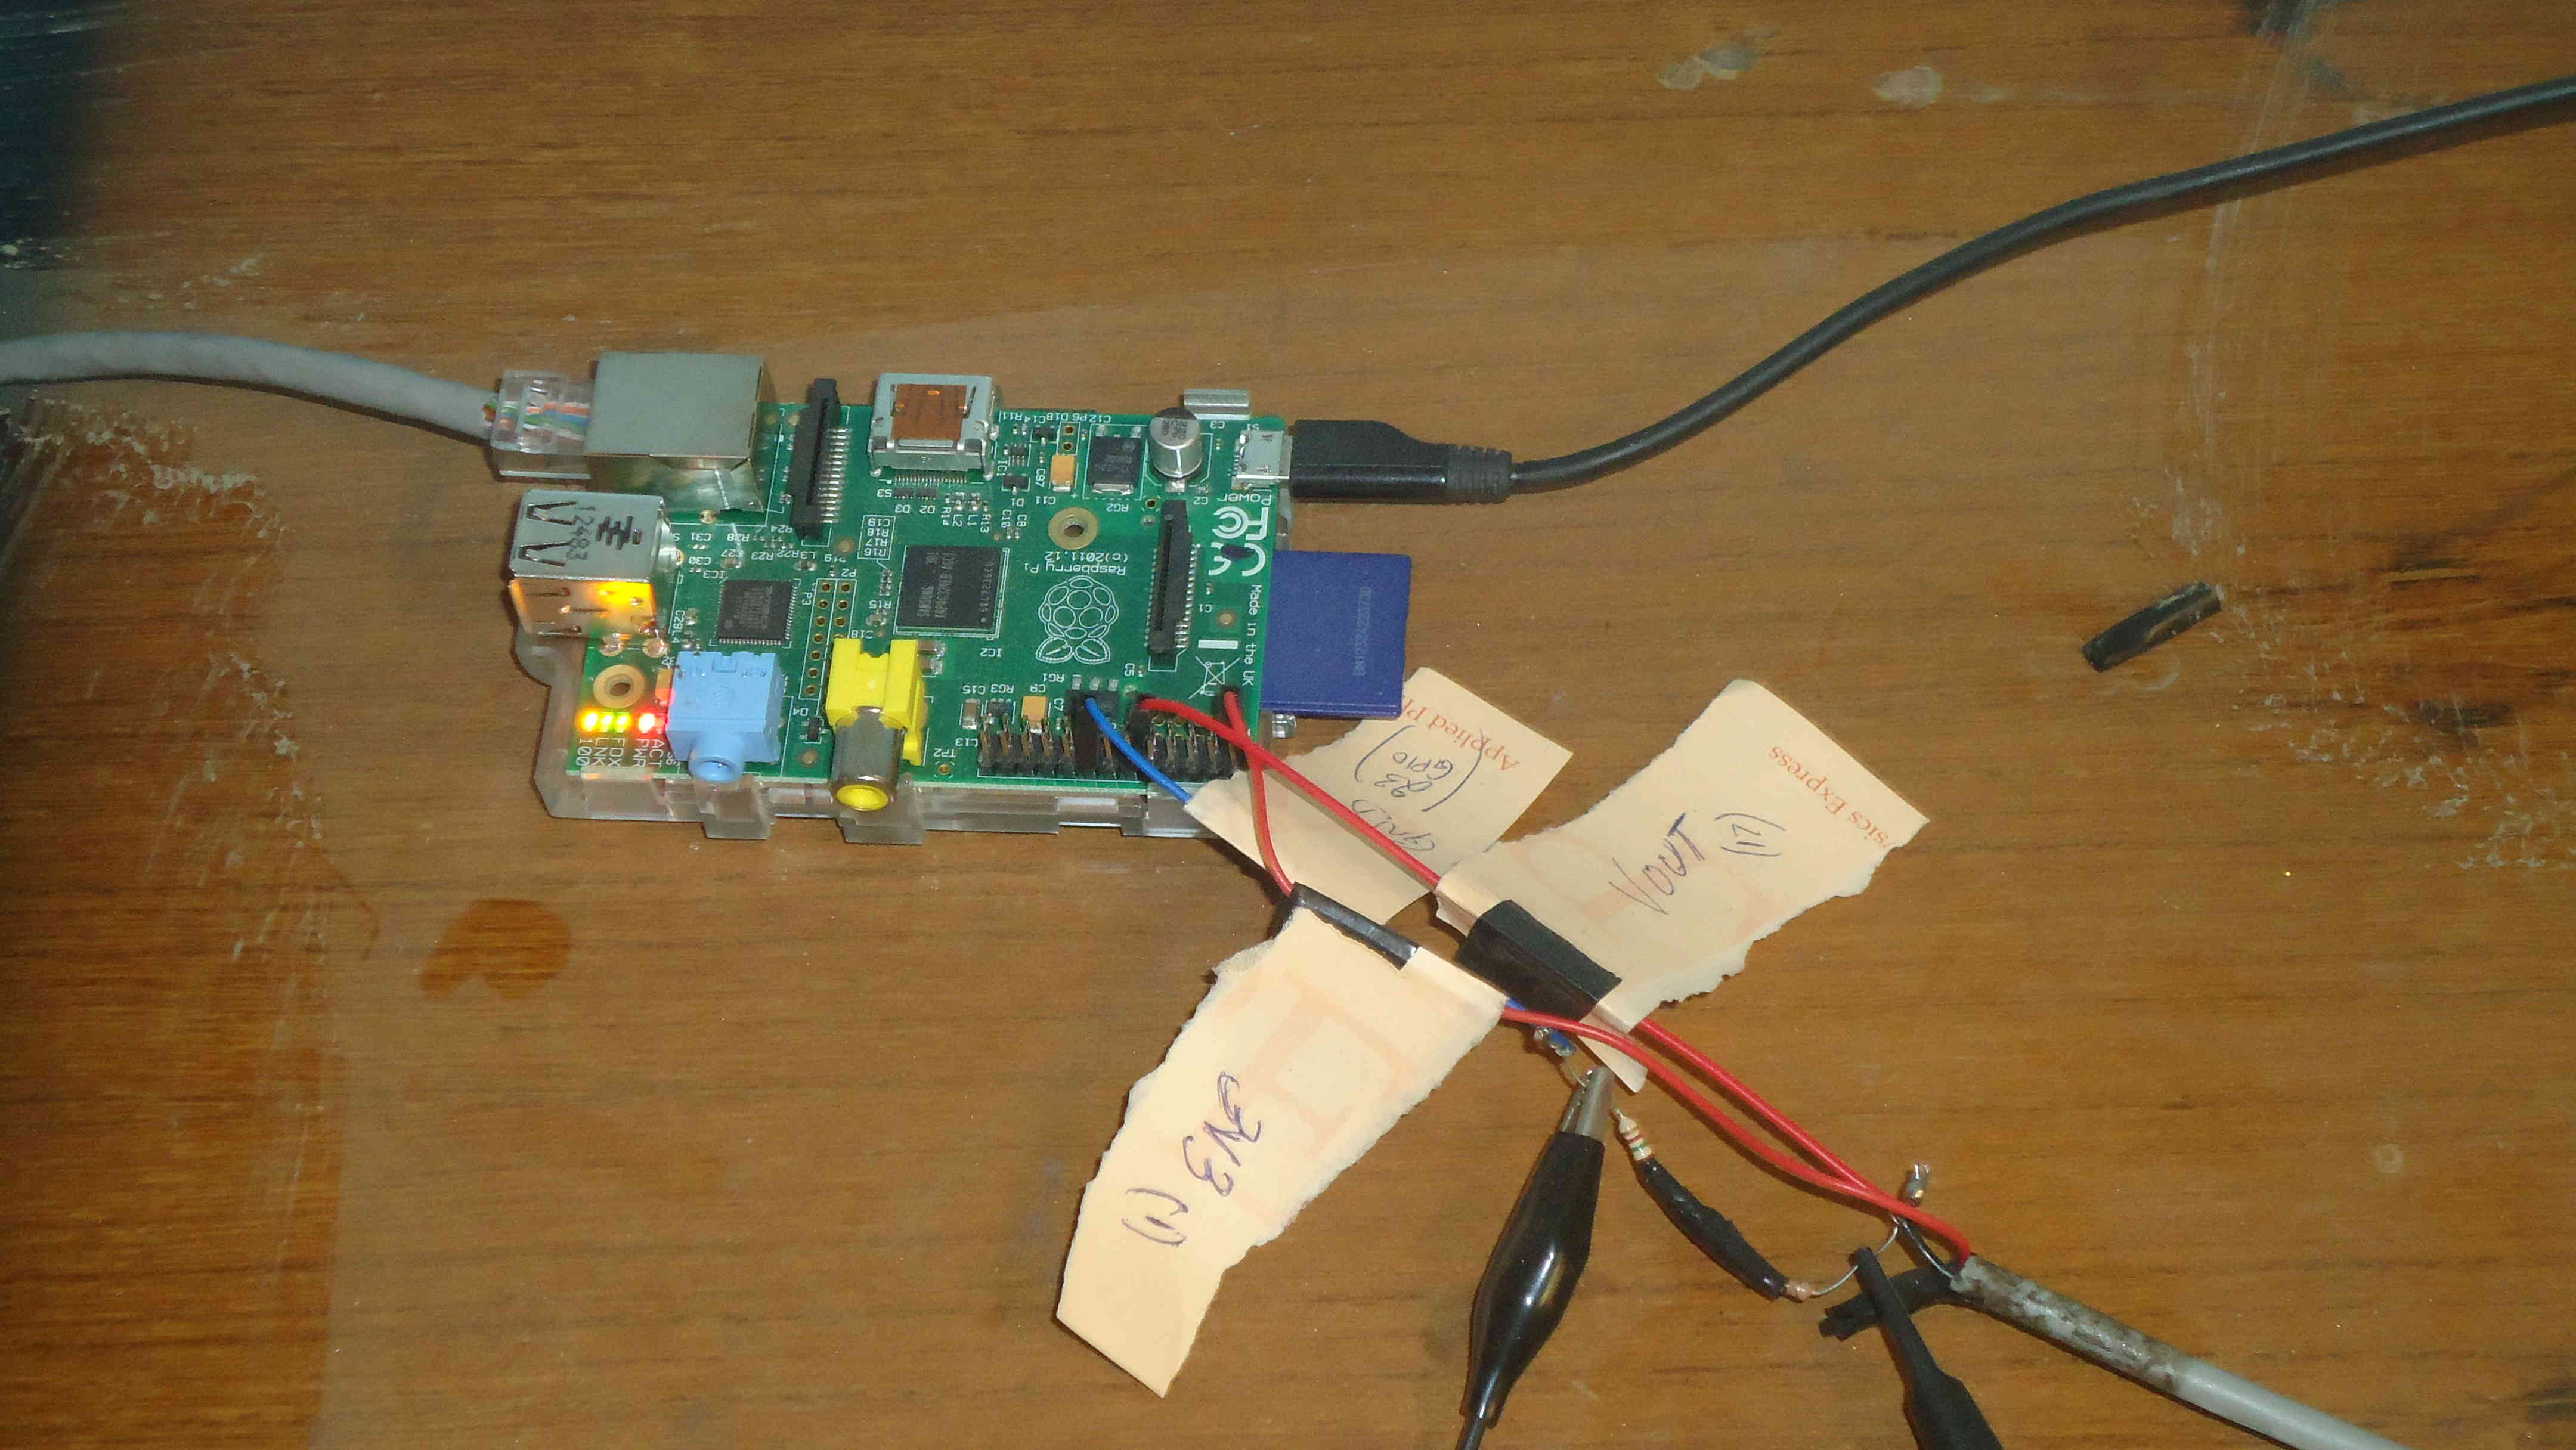
\includegraphics[scale=0.027]{./figures/rpi.jpg}}

    \caption{Sensing, computation and communication equipment used for deployment}

    \label{fig:deployment}

\end{figure*}

\section{How is this deployment different?}
\label{sec:learning}
In this section we discuss unique aspects brought forward from our deployment. Some of the key aspects are as follows:


\noindent \textbf{Unreliable grid is commonplace:} Load shedding or rolling blackout are common in developing countries, owing to several reasons such as improper infrastructure management, high demand and low electricity production. Power cuts are more common in summers when load is higher due to usage of air conditioners. As a result, voltage fluctuations or brownouts are also common. \figref{fig:failure_duration} shows power cut in number of hours per day during a two month period in summer of 2013. Electricity outage for upto 12 hours has been reported on some days. \figref{fig:failure_duration} shows the duration in minutes of power outages. 107 power outages were found in 61 day period from May to July. While the average power outage lasted about 1 hours, there were outages lasting upto 9 hours. \figref{fig:failure_hour} shows the power outage distribution by hour of the day. It can be seen that there are maximum outages around 10 AM in the morning and around midnight. These times correspond to office time and night time when air conditioners in home are on. We believe that this indicates heavy load on the grid. \figref{fig:voltage} shows the voltage fluctuations in a typical day, where it can be seen that voltage is fluctuating from 180 to 250 Volts. We can observe that voltage drops during peak load hours. This is in coherence with previous work\cite{nplug}, which hypothesized that frequency and voltage indicate load on the grid. \figref{fig:frequency} shows fluctuation in frequency in a typical day.

\noindent Due to unreliable nature of grid, we ensured that all our systems were capable of automatically starting after a power outage. We put our scripts for data collection and upload in Linux startup script. This provided us another advantage. If we observed that a system was down, we could just ask the home occupant to repower the system again. This ensured that there was minimal data loss till the time our researchers could visit the site and repair the fault.


\noindent \textbf{Unreliable internet connectivity:} While India has one of the fastest growing internet population, only 11 \% of the total population is connected to internet, while the corresponding figure in US is 78\%\cite{meyer}. Average connection speed in India is 1.3 Mbps, the corresponding numbers in developed countries are in excess of 10 Mbps\cite{state_of_internet}. Even though the condition of interent has vastly improved, from practical experience, we have found it to unreliable. We found internet would be unavailable several times during the day and sometimes it would be too slow.
Homes have poor connectivity. This forced us to develop a different paradigm which we call Sense-Store-Transfer. This is shown in \figref{fig:network}


\begin{figure}
\subfloat[\scriptsize Before repair]{
    \label{fig:before_repair}
    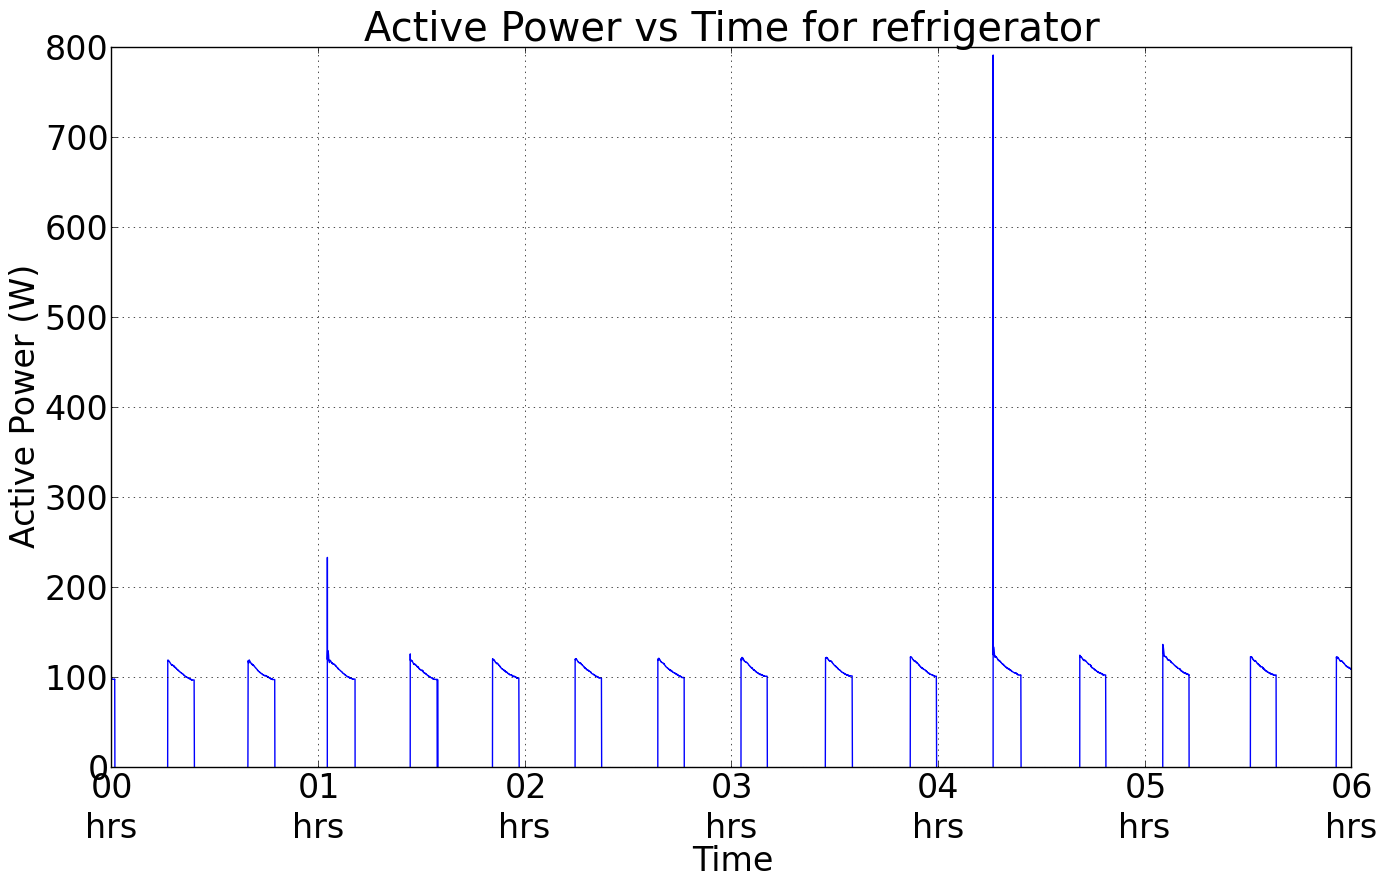
\includegraphics[scale=0.12]{./figures/before_repair.png}}
     \subfloat[\scriptsize After repair ]{
        \label{fig:after_repair}
        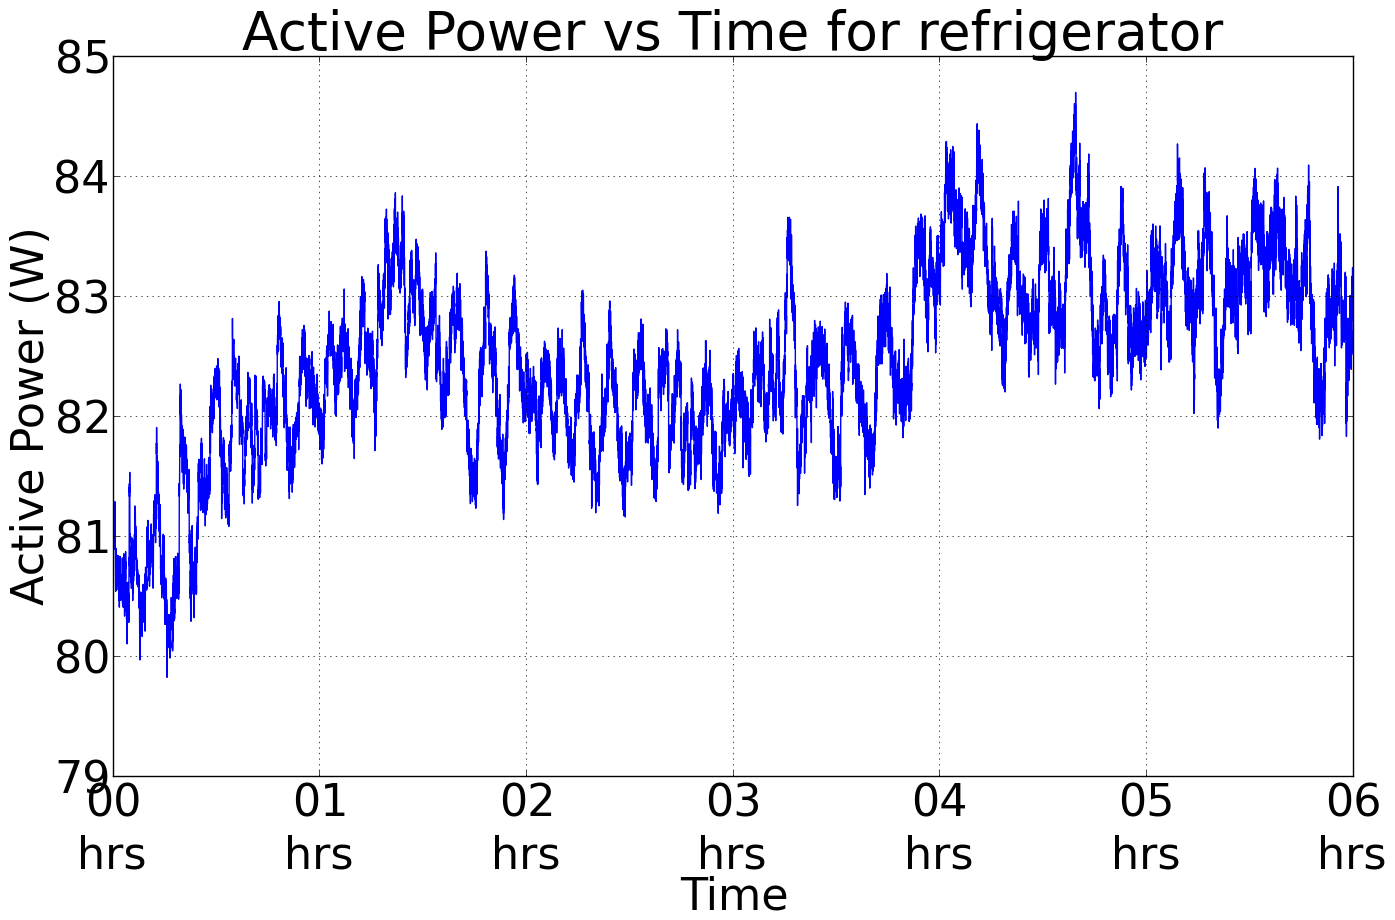
\includegraphics[scale=0.12]{./figures/after_repair.png}}
       
   
    \caption{Refrigerator power consumption}

    \label{fig:metadata}

\end{figure}
	
\noindent \textbf{Importance of meta data collection:} We collected metadata associated with electrical appliances throughout our deployment. We collected parameters such as appliance name, age, mode of usage (for instance air conditioner set temperature). We believe this detailed metadata can enhance NILM and can provide useful insights for conserving electricity. For instance, in one of the home refrigerator was sent for repairing on 2$^{nd}$ July. \figref{fig:before_repair} and \figref{fig:after_repair} show the active power consumption before and after repair. We found that after repair the refrigerator was configured in coolest mode (lowest temperature), while before repairing, it was configured in least coolest mode (highest temperature). After repair the refrigerator was found to be consuming 1KWh more. Moreover, its duty cycle pattern was modified significantly. This metadata can be useful to NILM approaches which model appliance usage duration as one of their parameters.

\noindent \textbf{Load specifics:} Electrical load setting in India are different from that in the US and Europe. There are no automated loads. HVAC systems are decentralized. Thus, air conditioning is at room level and water heating is done using geysers at bathroom levels. From our deployments we observed that air conditioners and geysers account for upto 70\% and 50\% of overall home electricity in summers and winters respectively. Thus, any small improvement in efficiency of these two appliance can significantly lower the home electricity consumption.

\noindent There are also special appliances such as water motor and water filter, owing to which there is energy embedded in water. Water motor, earlier described in section \secref{sec:sensing}, is used to pump water upto water tank on roof. It was observed that without motor it took 8 seconds to fill 1 liter of water into the tank and after switching on the motor it took 4 seconds. Also, water filter 

\noindent \textbf{Lack of quality measurement devices commonly found in US and Europe:} ZWave sensors for Indian frequency (865.2 MHz) are not available. Thus, we imported from European frequency (868.4 MHz) based ZWave multisensors and plug load monitors. Import duty and shipment delays make them an expensive choice. As explained above, ZWave based plug load monitors could not be used in our deployments, since they need to be explicitly turned ON. Further other alternatives like Current Cost based CT's would involve exposing live wire from appliances, an option which was rejected by home occupants. Thus, we had to resort to jPlug, which is a prototype solution.

\section{Hitchiker's guide revisited}
\label{sec:common}
In this section, we discuss similarities between our deployment and those explained in previous work. We further explain how we tackled these issues. Some prominent similarities are:

\noindent \textbf{Homes are hazardous environments:} We observed that one of our multisensors would fail after power outage. Initially, we felt that the sensor was faulty, but when other sensors showed the same behavior in the same location. We figured that this behavior was due to the fact that this multisensor was put on inverter point (battery backup) and would not go down even on power outage. Thus, when power resumed, ZWave controller was not able to add this multisensor to its network. We resolved this by putting the multisensor at a non-inverter point. We also observed that one of the multisensor always indicated motion. We were able to solve this problem primarily by replacing its power supply. However, within a week this problem resurfaced. We believe it is due to faulty power supply in that room. The home occupants did not allow a thorough investigation of that electrical socket and we had to do away with that data.

\noindent Although we took caution of using zip-ties to prevent hanging wires, we observed data loss in one of our multisensor and Android phones, which went out of power due to wire snag. This is shown in \figref{fig:snag}. Further, even after 1 month rigorous testing in lab, we found that 60 new issues (service complaints) were registered when we moved the deployment to the first home. This is only a testimony that homes present a unique scenario which can not be emulated well in laboratory settings.

\noindent \textbf{Aesthetics matter:} As stated in previous work, sensor LED's can be bothersome to home occupants, particularly in the night. Our 33 sensor deployment had introduced 63 LED's in the home. \figref{fig:led} shows our sensor LED's blinking in the night. For our current deployment, choosing appropriate sensor location sufficed. However, for future such deployments, we intend to build better casing. Also, the home occupants complained of buzz like sound coming from the desktop server that we had put. We figured that this noise was due to the fact that its CPU was clogged due to dust. This is another unique aspect introduced in the Indian setting. Thus, any long lived deployment should have routine maintenance.

\noindent \textbf{Homes are not designed for sensing:} We observed that the data collected from our ground floor MCB's (5 in number) was noisy. This was due to the fact that the MCB's are very close (shown in \figref{fig:ct_interference}) to each other and this causes interference in our CT monitoring circuit. However, on the 3 MCB's on the first floor, there was adequate gap amongst MCB's and data was of good quality. We thus believe that homes are not designed for sensing and one should be prepared to lose some data quality due to that.

\noindent \textbf{Redundancy-Accounting for sensor failure:} During our deployment 3 jPlugs and 1 multisensor stopped functioning properly. Fortunately, we had accounted for such failure and had additional sensors ready. We believe that one should beforehand  account for sensor failure in residential deployments.

\noindent \textbf{Homes have poor connectivity:} During the preliminary phase of our deployment, we tried to work with existing networking infrastructure in the homes. The WiFi router was placed on the first floor and signal strength on ground and second floor was poor. \figref{fig:ground_without_router} and \figref{fig:second_without_router} show the WiFi heatmap produced wrt the router placed on first floor. We observed that a lot of regions show poor signal strength. We bridged an additional router on the ground and the second floor with the existing first floor router. \figref{fig:ground_with_router} and \figref{fig:second_with_router} show the corresponding WiFi heatmaps produced wrt newly introduced bridged routers. We can observe the improvement in signal strength with the introduction of additional hardware. 

\noindent Another important facet of deployments is that additional sensors introduced inside a home may choke up the bandwidth. We observed this when we tried using imported WiFi based microcontrollers for sensing ambient conditions. Home users complained of low bandwidth available for their personal usage and thus, we decided to use ZWave based multisensors for measuring ambient parameters. Since ZWave based sensors worked on a different frequency when compared to WiFi, they did not cause interference. Thus, in our experience, a careful mix of sensors working on different frequencies should be used to avoid interference issues.

\begin{figure}  
\subfloat[\scriptsize Ground floor WiFi Heatmap without additional router]{
	 \label{fig:ground_without_router}
    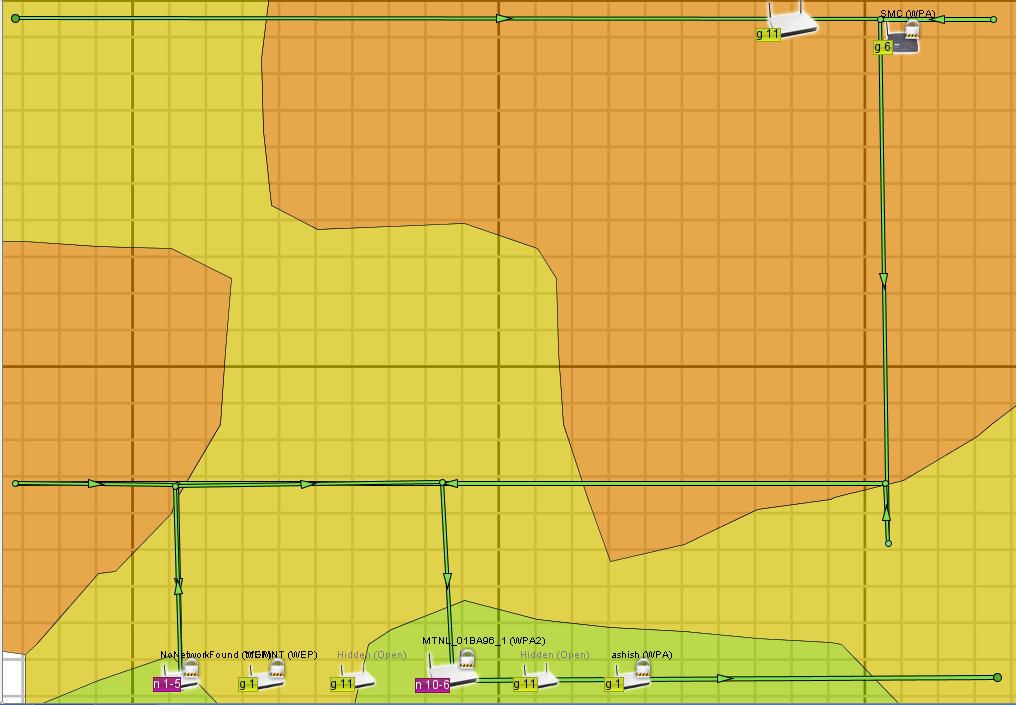
\includegraphics[scale=0.11]{./figures/ground_without_router.png}}
    \hspace{1mm}
    \subfloat[\scriptsize Ground floor WiFi Heatmap with additional router]{
    	 \label{fig:ground_with_router}
        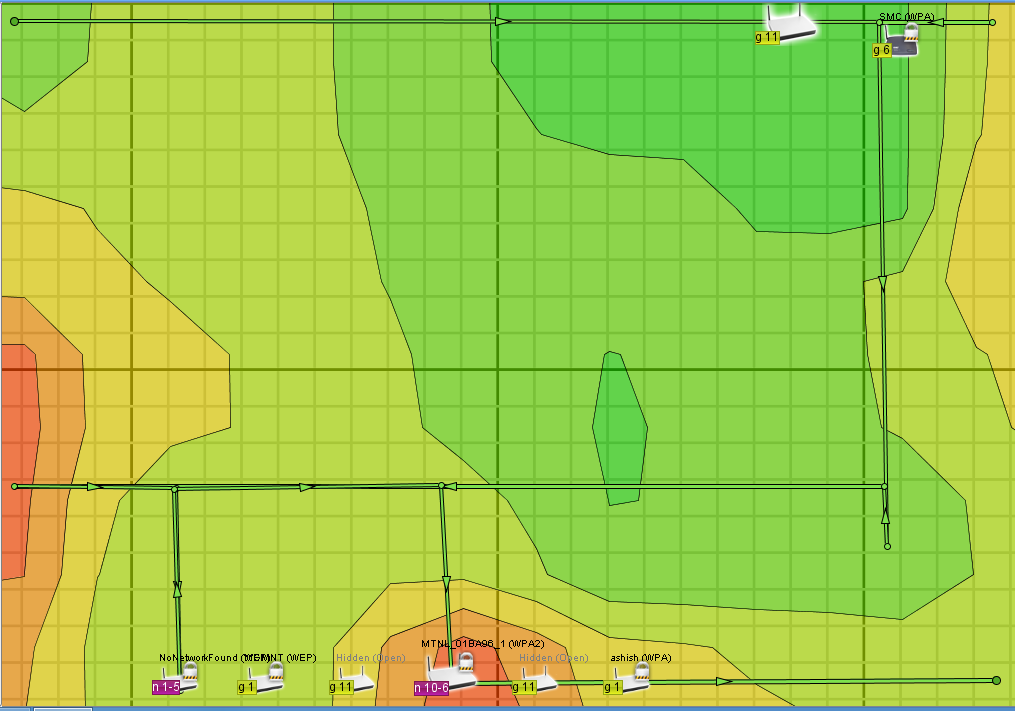
\includegraphics[scale=0.11]{./figures/ground_with_router.png}}
       \newline
      \subfloat[\scriptsize Second floor WiFi Heatmap without additional router]{
      	 \label{fig:second_without_router}
          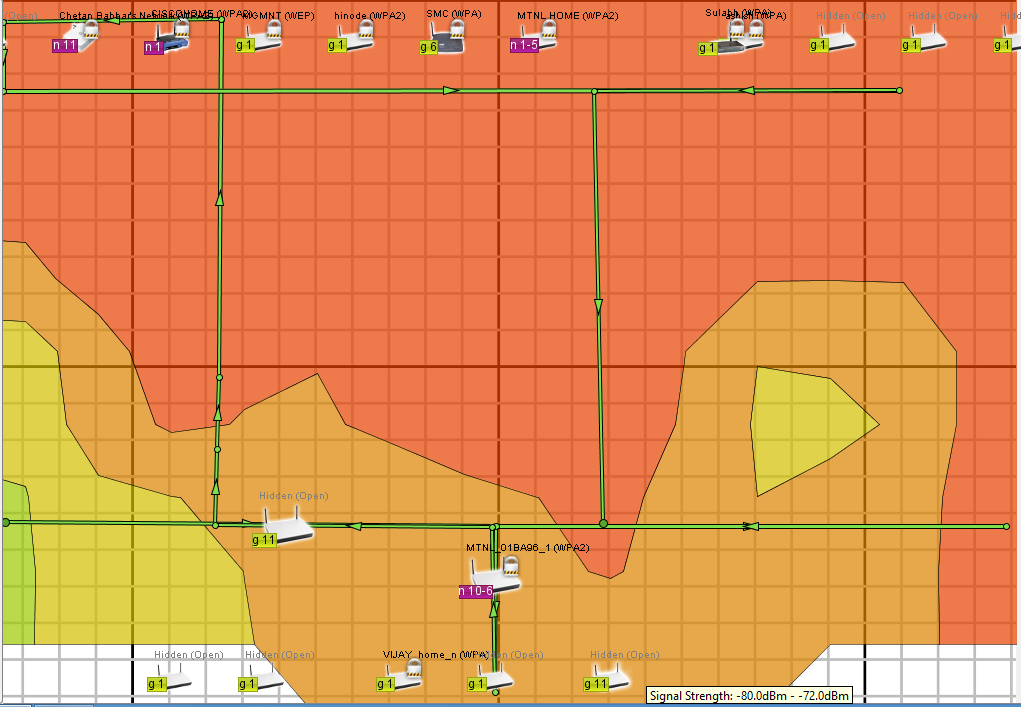
\includegraphics[scale=0.11]{./figures/without_.png}}
          \hspace{1mm}
          \subfloat[\scriptsize Second floor WiFi Heatmap with additional router]{
          	 \label{fig:second_with_router}
              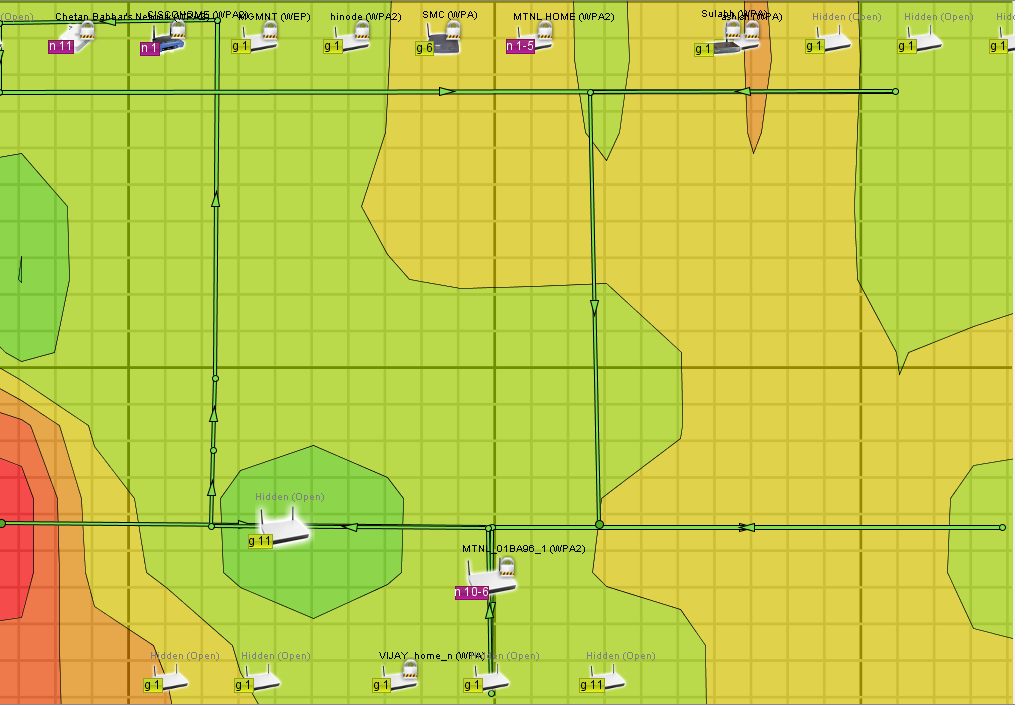
\includegraphics[scale=0.11]{./figures/with_.png}} 
    \caption{WiFi signal without placing additional routers on different floors is poor. The greener the region, the better the signal strength for the heatmap.}   
      
\end{figure}




\begin{figure*} 
    
    \subfloat[\scriptsize Power outage vs Time]{
    \label{fig:failure_time}
    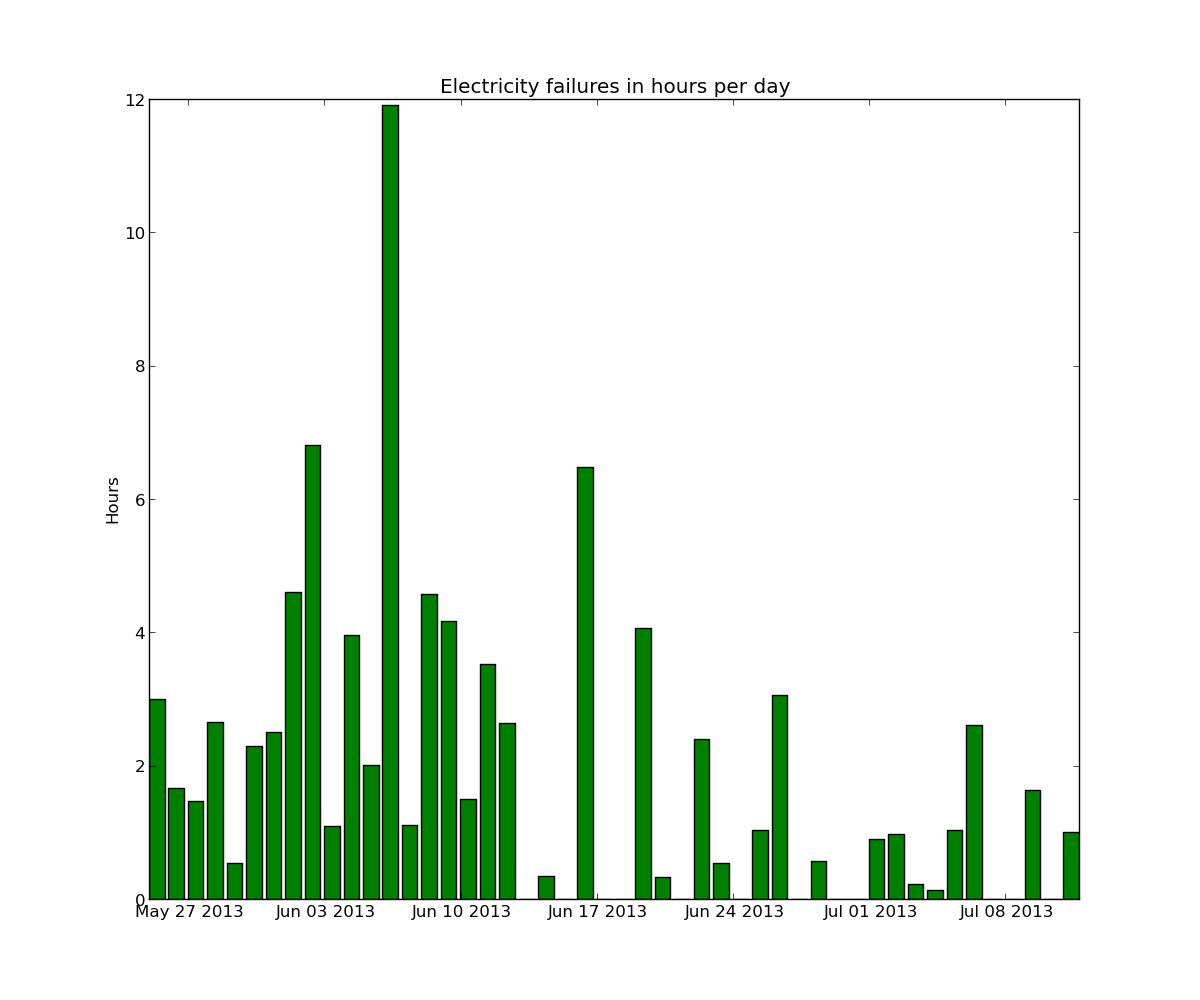
\includegraphics[scale=0.15]{./figures/electricity.png}}
    \hspace{1mm}
     \subfloat[\scriptsize Power outage durations ]{
        \label{fig:failure_duration}
        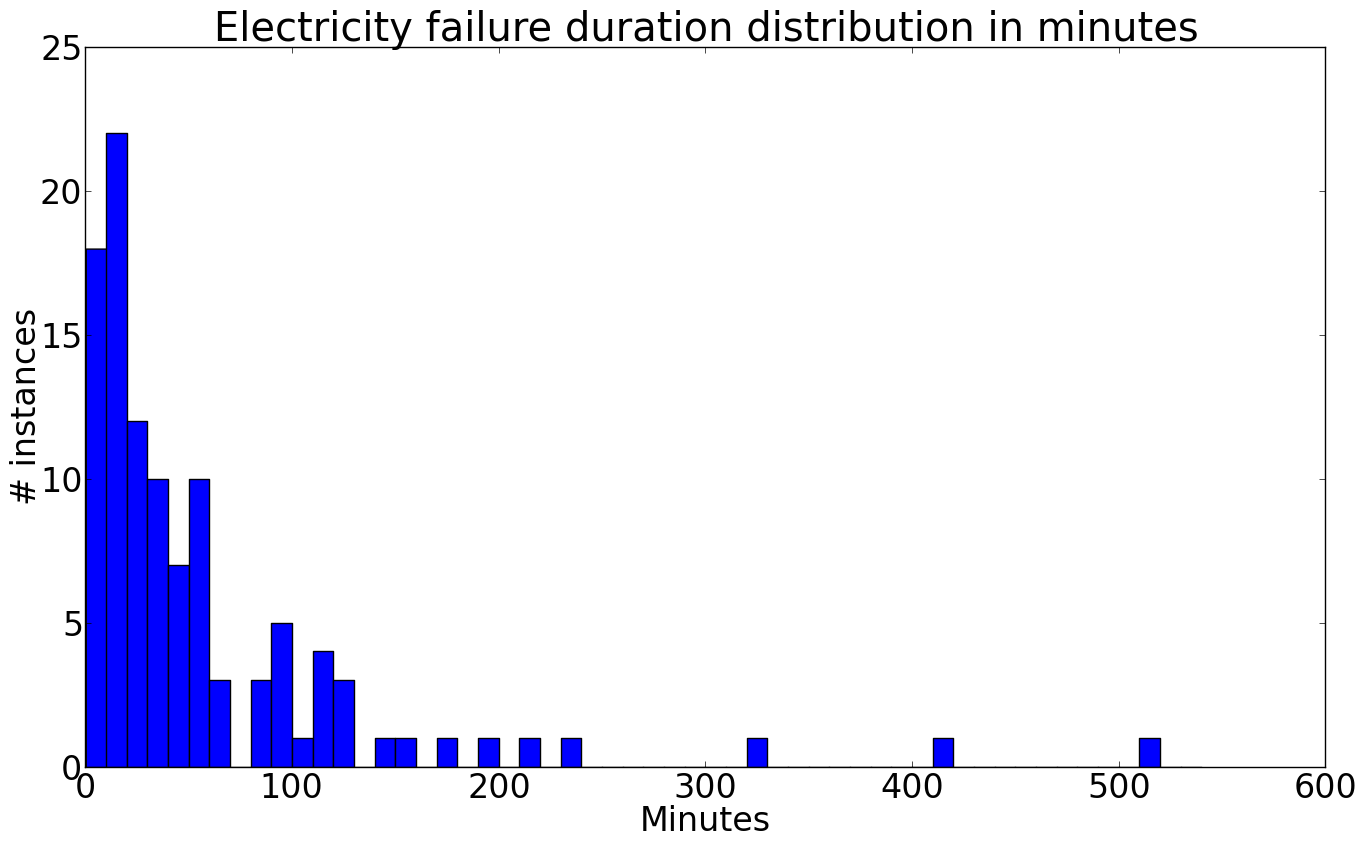
\includegraphics[scale=0.15]{./figures/failure_durations.png}}
       \hspace{1mm}
     \subfloat[\scriptsize Power outage by hour of day]{
             \label{fig:failure_hour}
             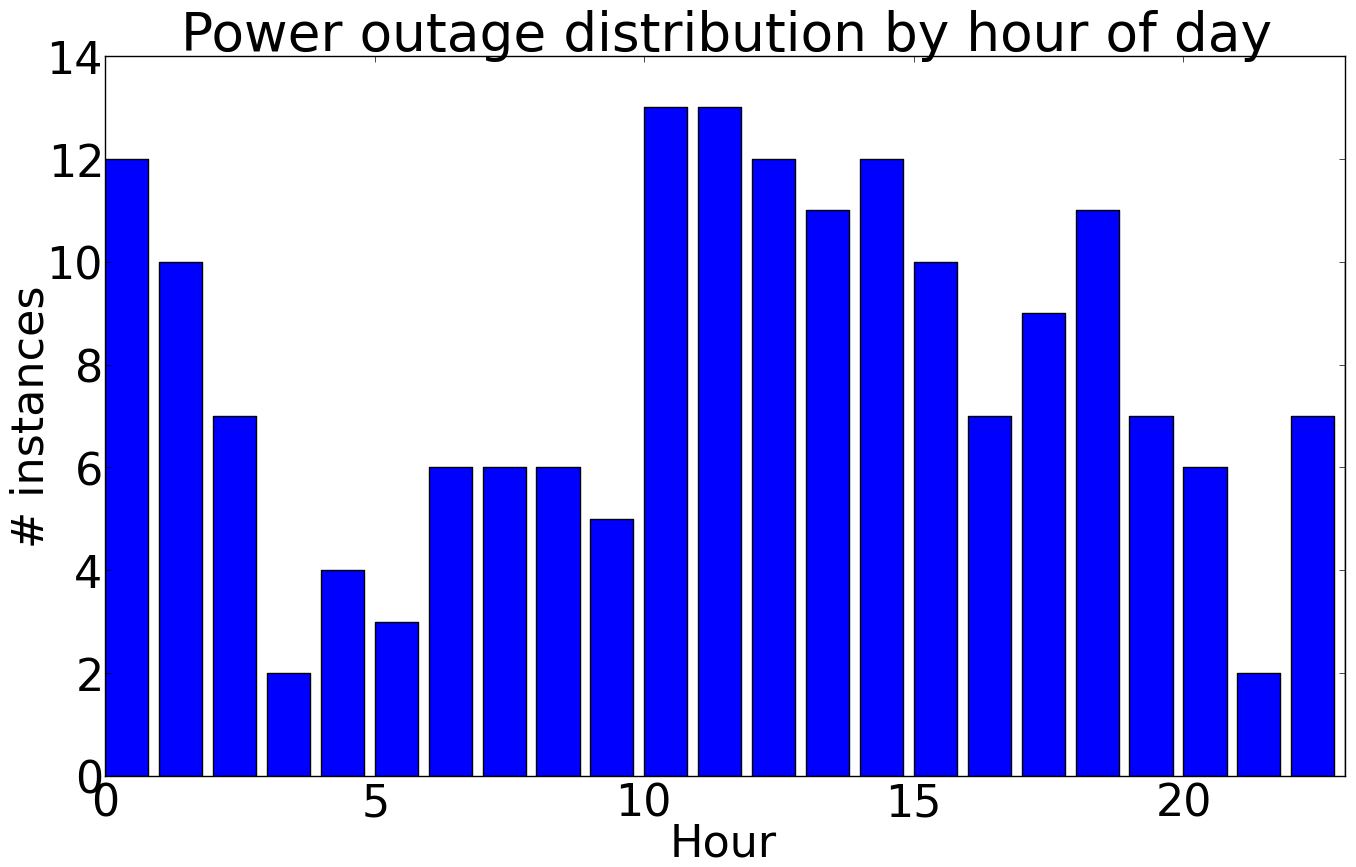
\includegraphics[scale=0.15]{./figures/outage_by_hour.png}}
              \vspace{-4mm}
             \newline
            
          \subfloat[\scriptsize Voltage fluctuations in a typical day. Rated voltage is 230 V]{
                  \label{fig:voltage}
                  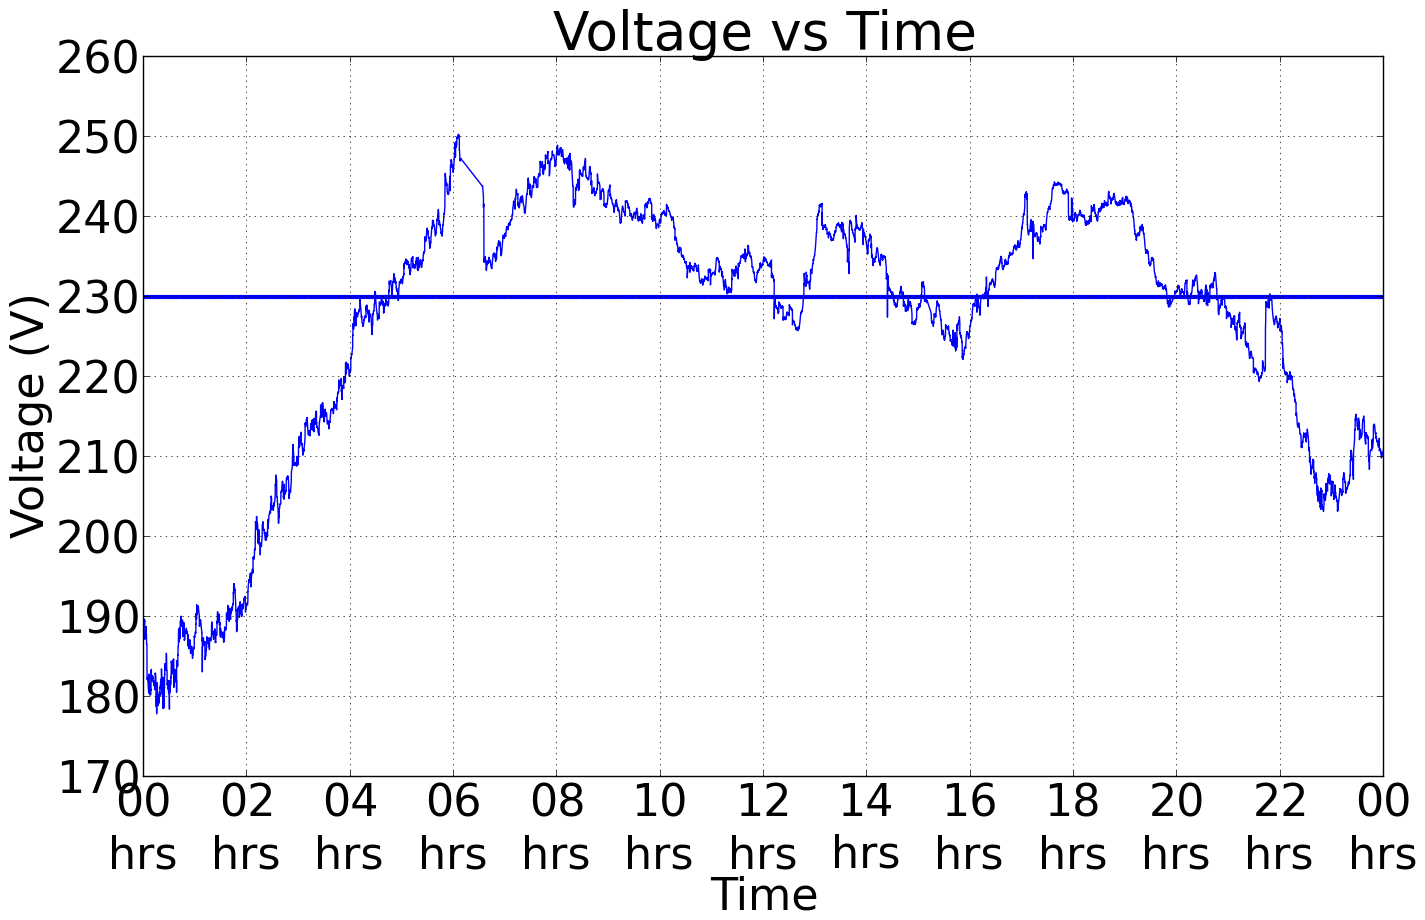
\includegraphics[scale=0.15]{./figures/voltage.png}}
          \subfloat[\scriptsize Frequency fluctuations in a typical day. Rated frequency is 50 Hz]{
                            \label{fig:frequency}
                            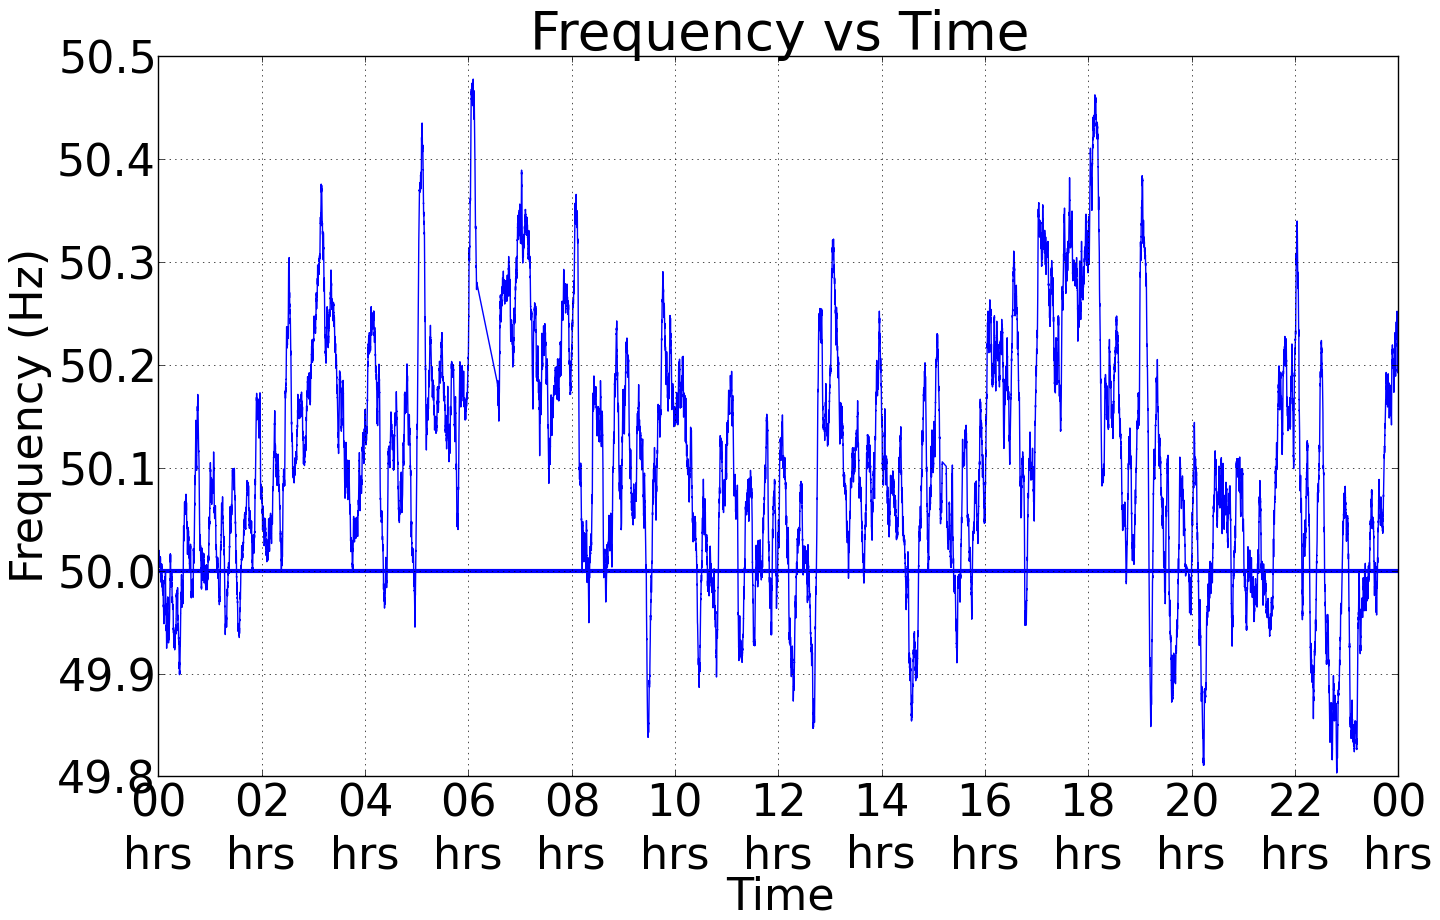
\includegraphics[scale=0.15]{./figures/frequency.png}}
          \subfloat[\scriptsize \% internet packet drop]{
                            \label{fig:network}
                            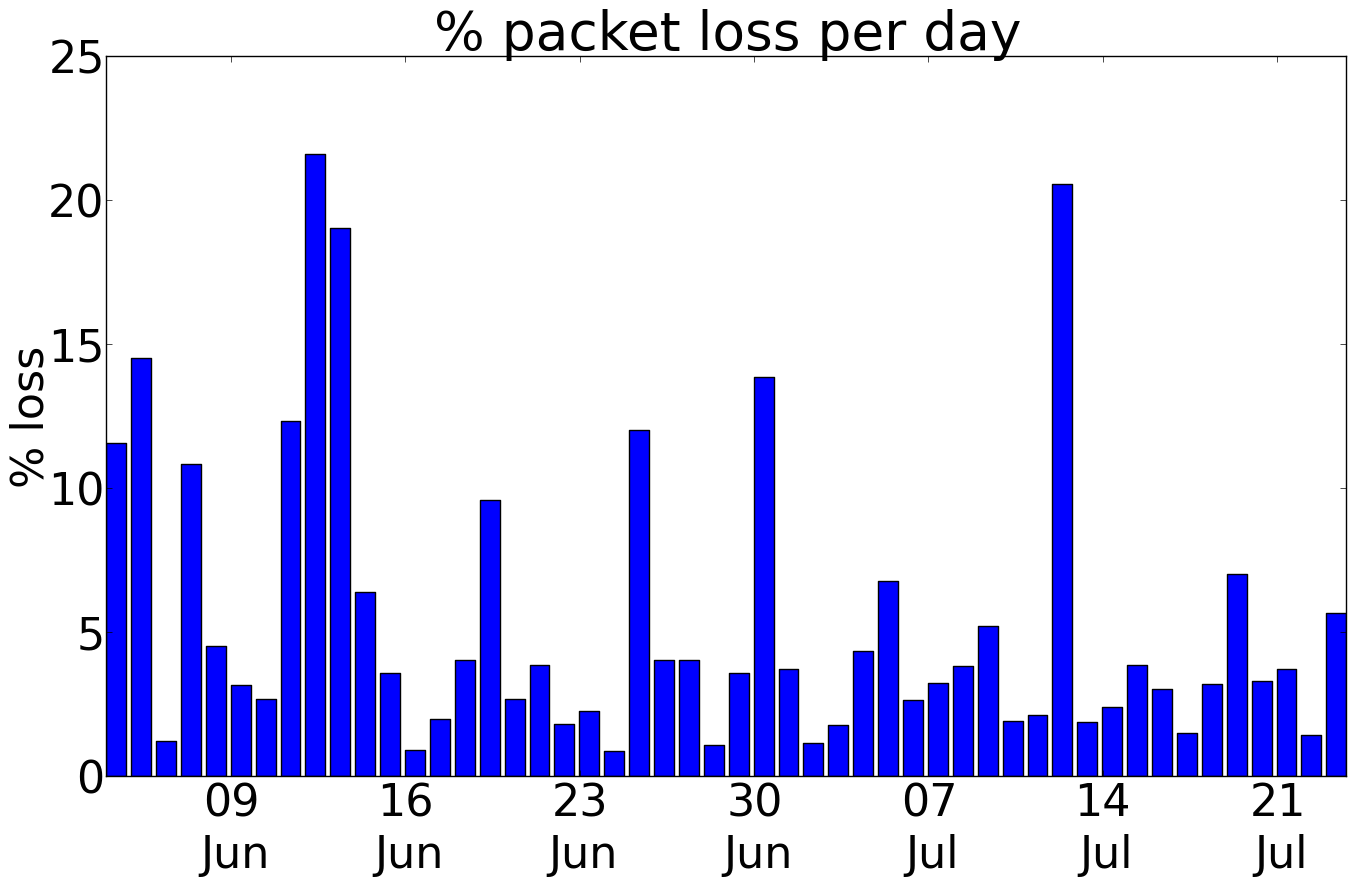
\includegraphics[scale=0.15]{./figures/network.png}}
   
    \caption{Unreliable internet and grid}

    \label{fig:unreliable}

\end{figure*}

\begin{figure}     
    \subfloat[\scriptsize Glowing LED's in night]{
        \label{fig:led}
        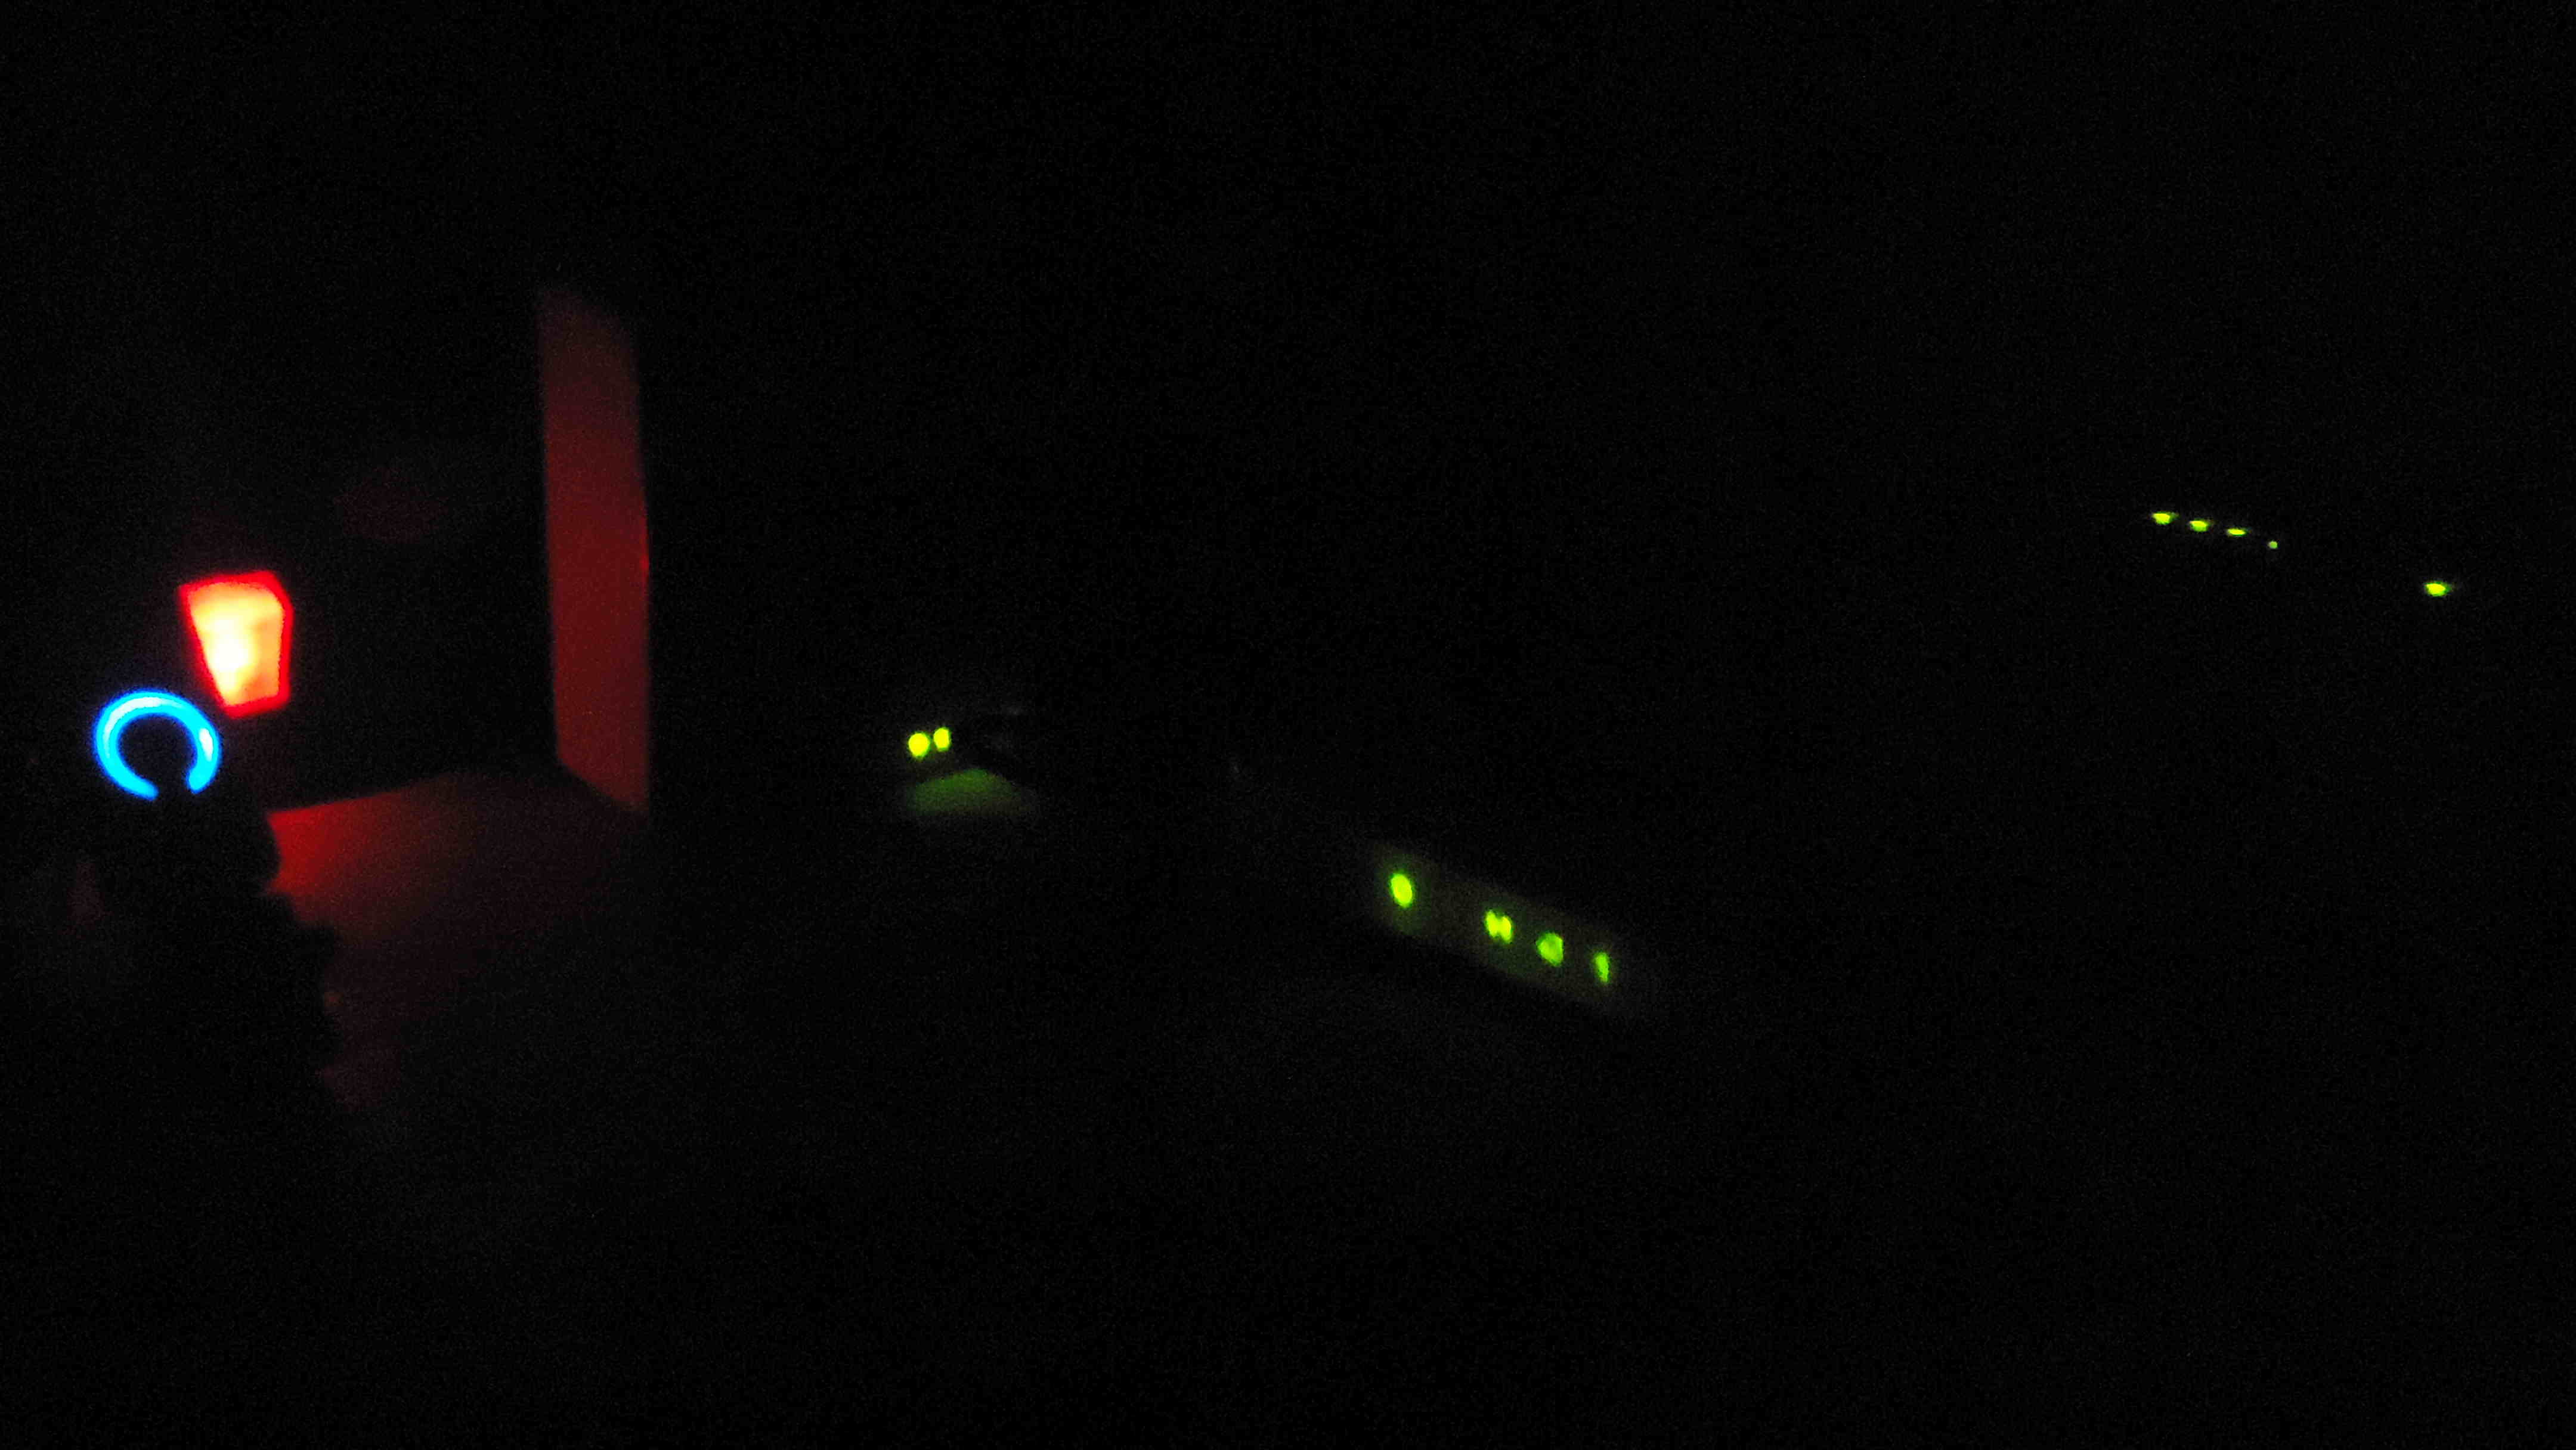
\includegraphics[scale=0.018]{./figures/led.jpg}}
        \hspace{0.1mm}
         \subfloat[\scriptsize Wire snag leading to data loss ]{
            \label{fig:snag}
            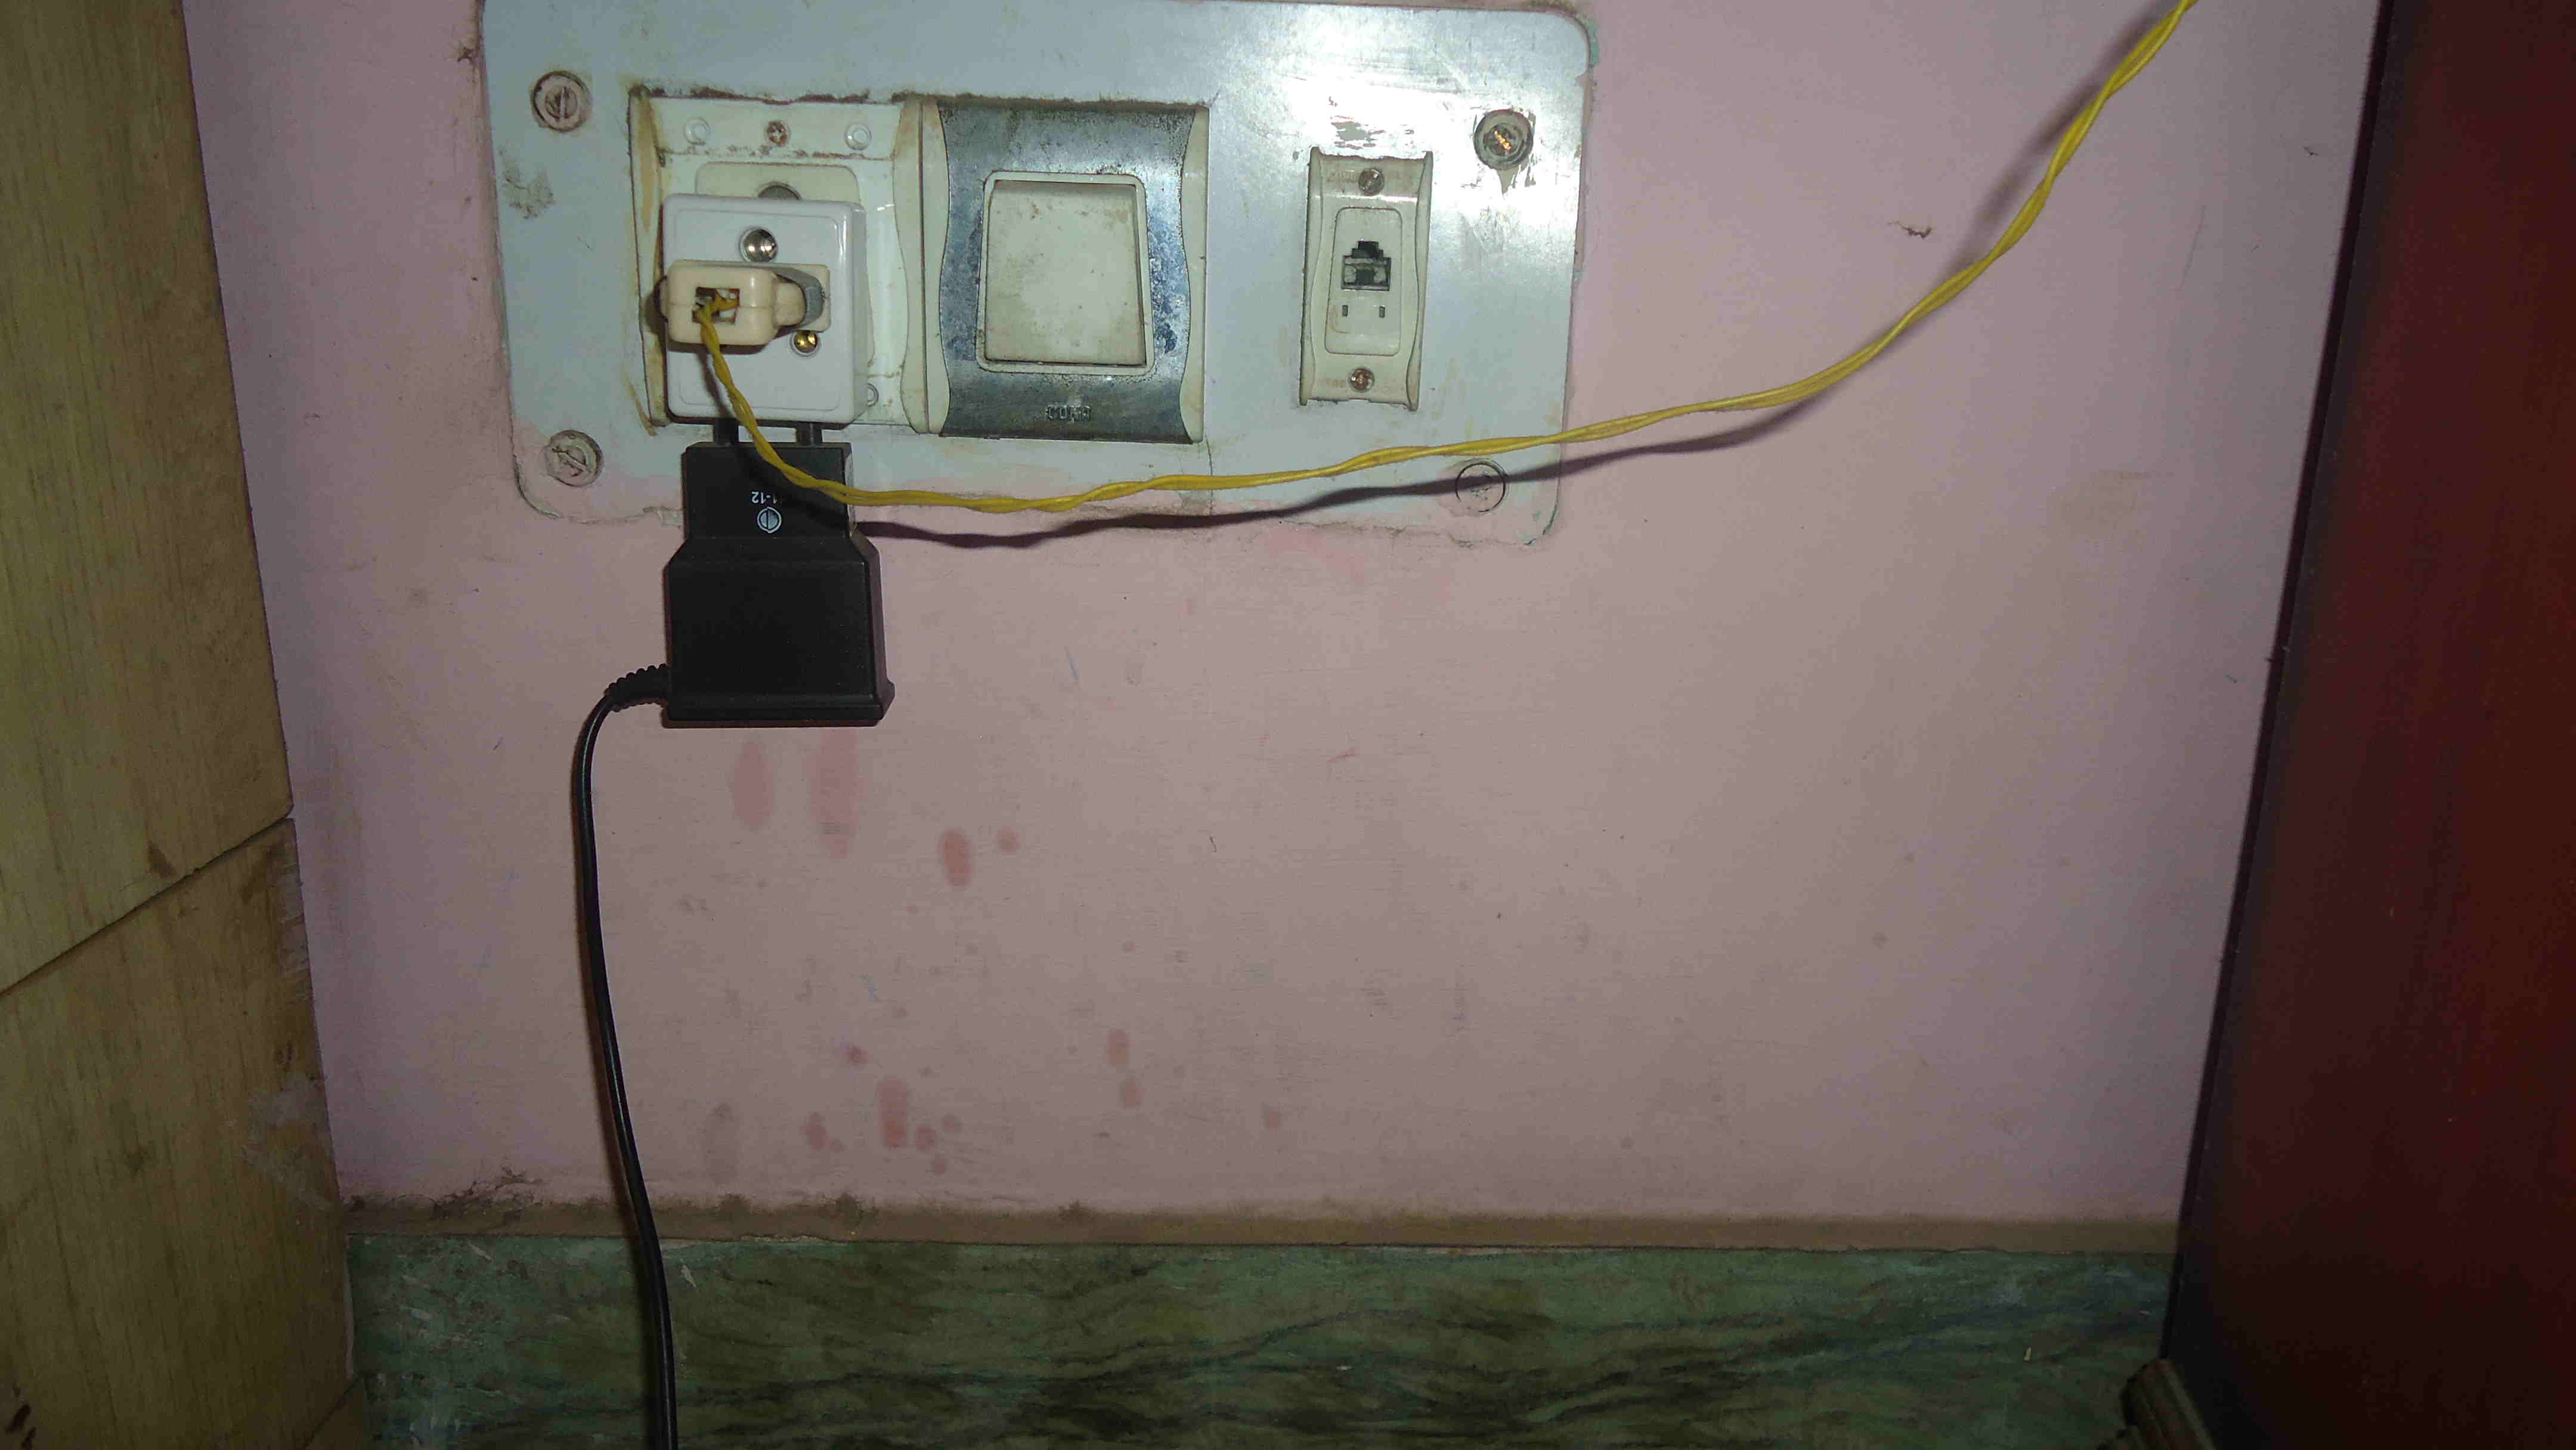
\includegraphics[scale=0.018]{./figures/snag.jpg}}
%                    \hspace{0.1mm}
        \subfloat[\scriptsize Closely placed MCB's causing interference in CT monitroing circuit ]{
                    \label{fig:ct_interference}
                    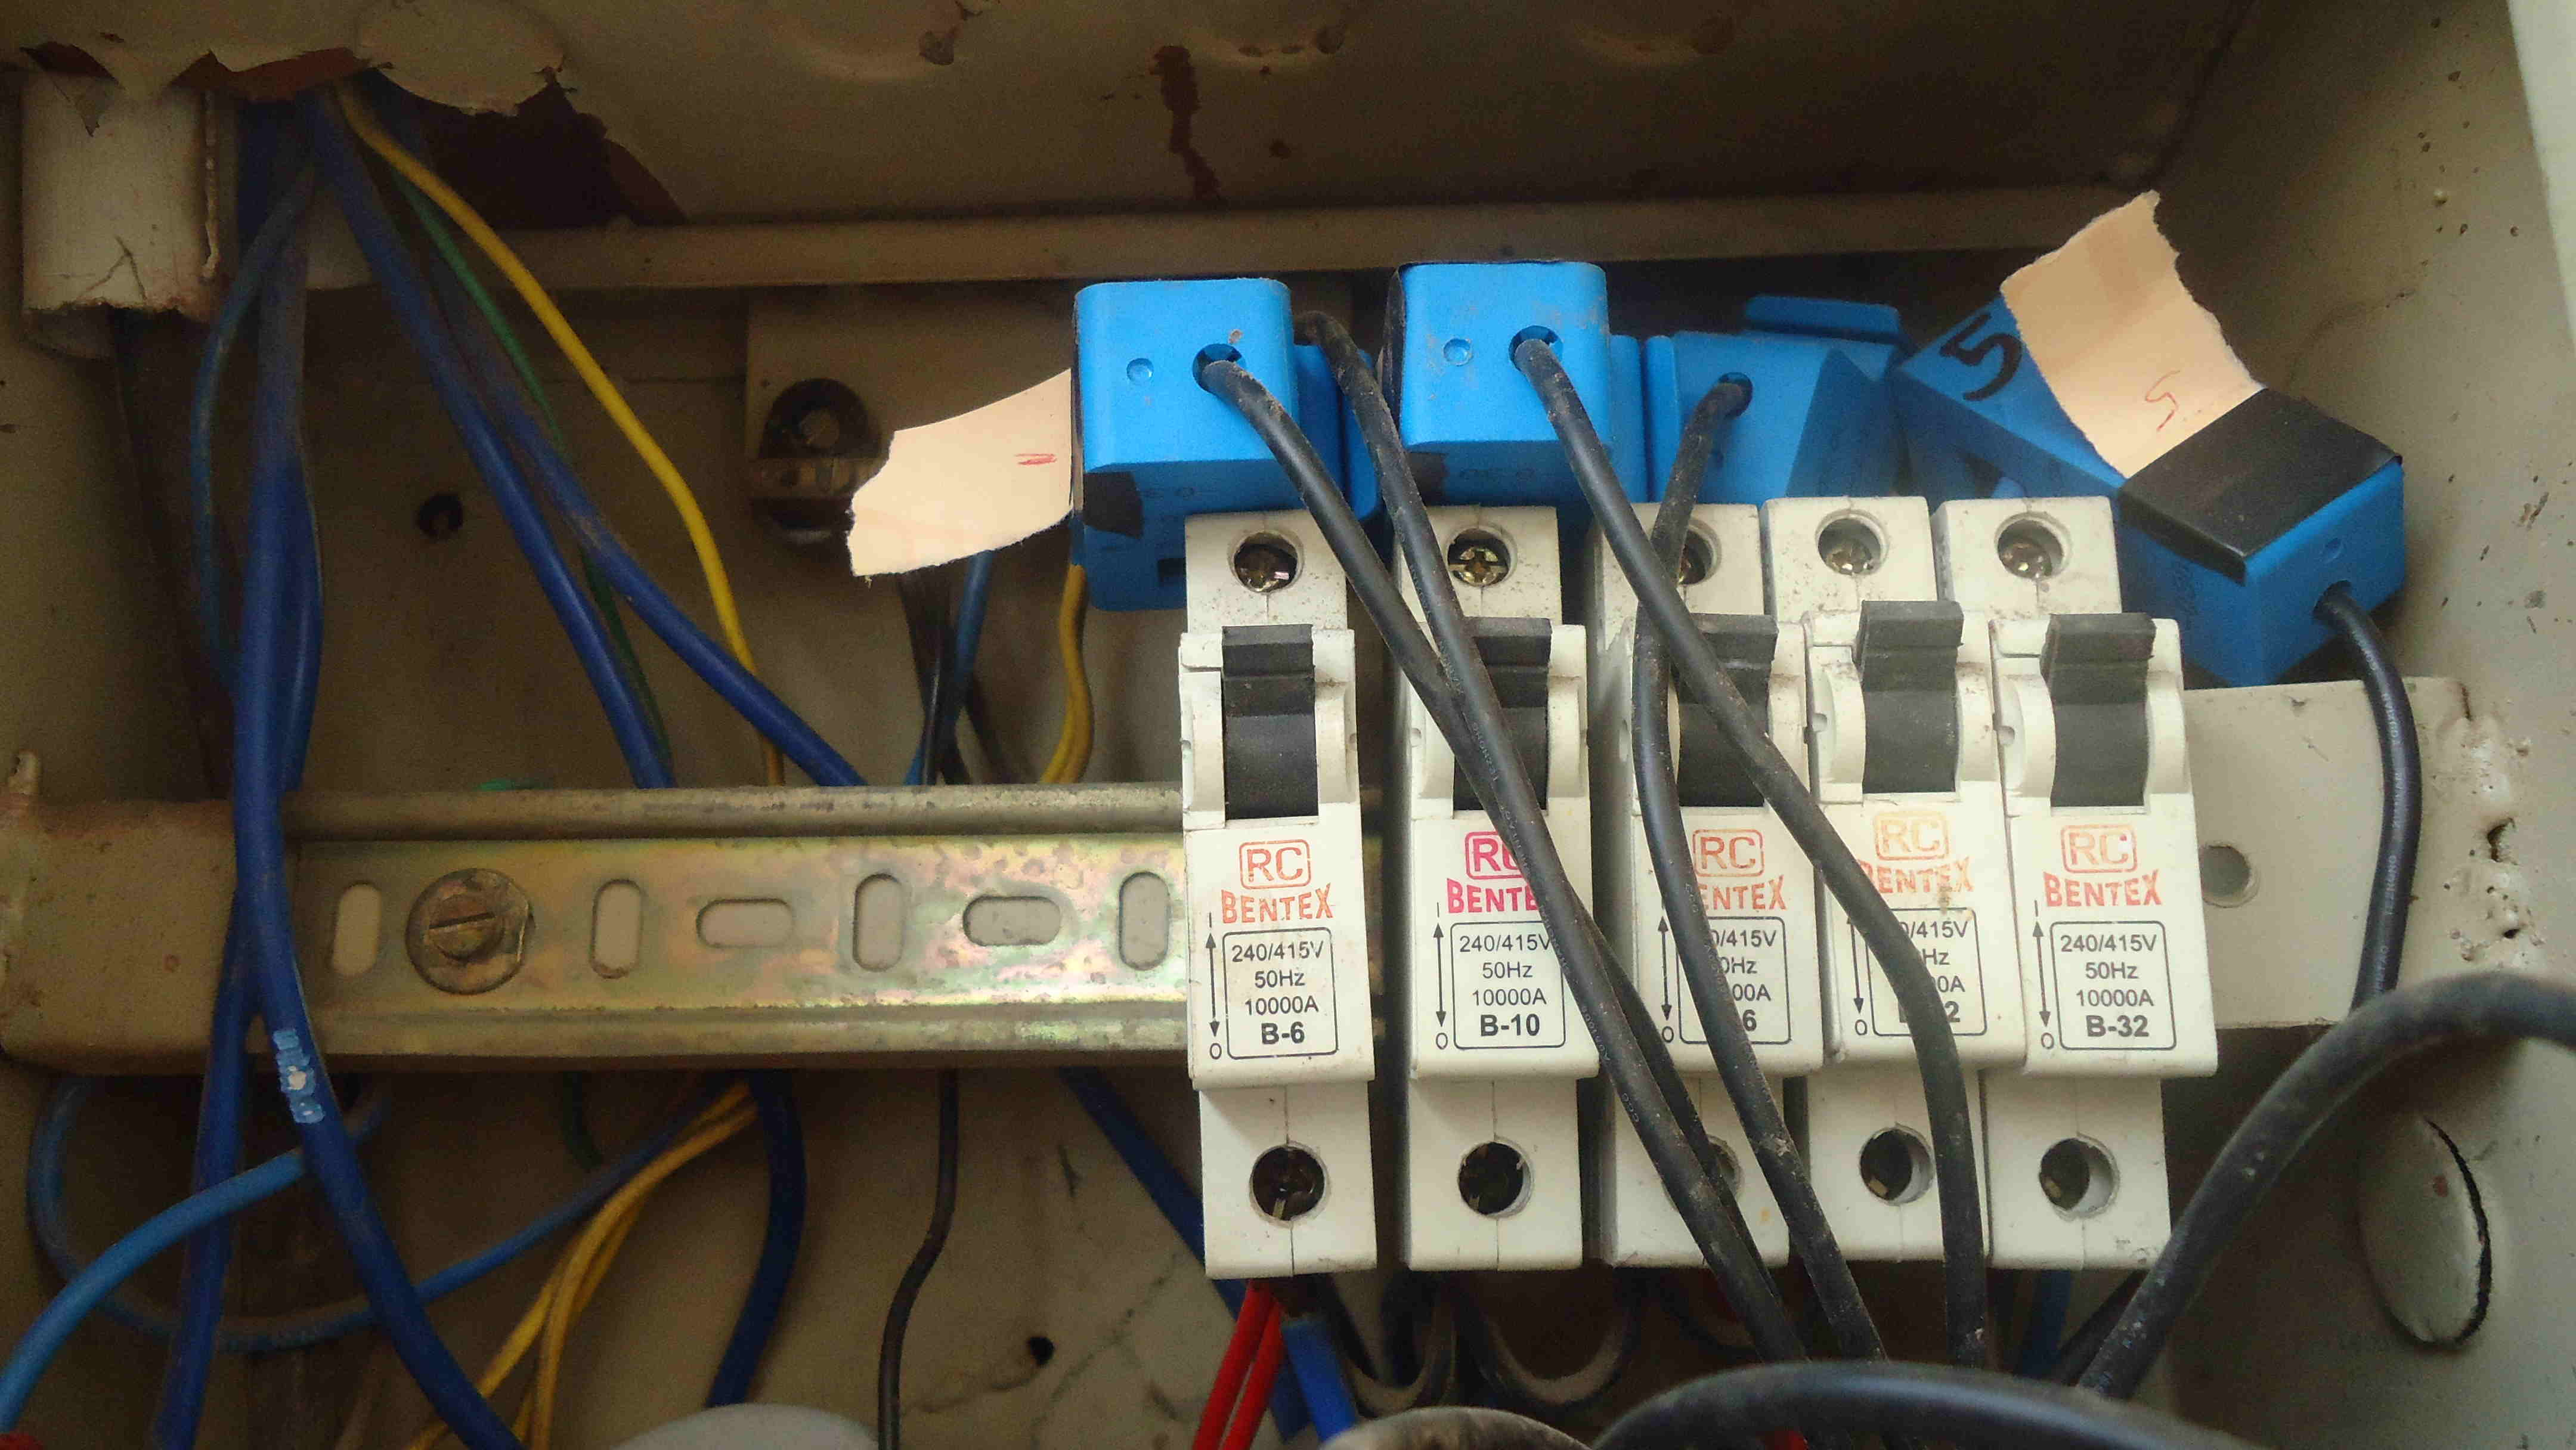
\includegraphics[scale=0.018]{./figures/ct_interference.jpg}}
    \caption{Common problems in residential deployments}   
    \label{fig:home}
   
\end{figure}


\section{Conclusions and Future Work}


\balance
\bibliographystyle{abbrv}
\bibliography{references}  % sigproc.bib is the name of the Bibliography in this case
\end{document}
